\documentclass[
version=last,
toc=bib,
toc=graduated,
toc=index,
toc=listof,
fontsize=9pt,
parskip=false,
openany]{scrbook}
%\pdfminorversion=4
\usepackage[utf8]{inputenc}
\usepackage[ngerman]{babel}
\usepackage{fontspec}
\usepackage[default]{sourcesanspro}
\setfontfamily\dejavuSansFont{DejaVu Sans}

\usepackage{ifmtarg}
\usepackage{ifthen}
\usepackage{etoolbox} % \ifstrempty

\usepackage{geometry}
\geometry{%a6paper
  paperwidth=125mm,
  paperheight=168mm,
  portrait,
  top=22mm,
  inner=22mm,
  outer=20mm,
  bottom=25mm,
  headsep=3mm,
  footskip=12mm
}

\usepackage{ragged2e} % nicer typesetting (hyphenation) for non raggedright and raggedleft
\usepackage{lscape}
\setlength{\parskip}{0pt}

\usepackage{relsize}

\clubpenalty=10000 %keine Schusterjungen
\widowpenalty=10000 
\displaywidowpenalty=10000 % keine Hurenkinder

\usepackage[]{microtype}

\usepackage{graphicx} % graphics

% search path for images
\graphicspath{{images-print/}{icons/}}
\usepackage{wrapfig}  % sponsor logos wrapped with text

\usepackage{tabu}
\usepackage{tabularx}
\usepackage{longtable}
\usepackage[table,cymk]{xcolor}
\usepackage{colortbl}

% embed PDF pages
% pdfpages must not be loaded before colortbl!
\usepackage{pdfpages}
% TikZ must not be loaded before colortbl
\usepackage{tikz}
\usetikzlibrary{calc}

% PDFs als Hintergrundbilder
\usepackage{multirow}
\usepackage{booktabs}
\usepackage{array}


\usepackage{refcount} % calculation of the page where the map is located

% page background
\usepackage[manualmark]{scrlayer-scrpage}
\pagestyle{scrplain}

\newcommand{\acro}[1]{{\textsmaller[0.5]{#1}}} % macro for abbreviations with more than one capitalised letter


% title/metadata
\title{FOSSGIS-Konferenz 2020}
\subtitle{Programm}
\author{FOSSGIS e.V.}
\date{\today}

\clearscrheadings

% page numbers
\cfoot[\begin{small}\pagemark\end{small}]{\begin{small}\pagemark\end{small}}
\ofoot[]{}
\ifoot[]{}
\pagestyle{scrplain}

% Durchschuss erhöhen
\linespread{1.15}

% include our custom macros
% command for a new time slot
\newcommand{\talkTime}{9:99}
\newcommand{\newTimeslot}[1]{\newpage\renewcommand{\talkTime}{#1}}

% new time slot but without a pagebreak
\newcommand{\newSmallTimeslot}[1]{\renewcommand{\talkTime}{#1}}

% initialise \conferenceDay 
\newcommand{\conferenceDay}{Noday}


\newcommand{\whitePageFill}{%
  \fill [white] (0,0) rectangle (125,168);
}

\newcommand{\drawCropMarks}{%
  \draw (10,0) -- +(0,5);
  \draw (0,10) -- +(5,0);
  \draw (115,0) -- +(0,5);
  \draw (125,10) -- +(-5,0);
  \draw (10,168) -- +(0,-5);
  \draw (0,158) -- +(5,0);
  \draw (115,168) -- +(0,-5);
  \draw (125,158) -- +(-5,0);
}

% macro to expand to TikZ code to render the day label
% 1. day
% 2. y offset of coloured box from bottom
% 3. y offset of text label from bottom
\newcommand{\dayLabelRight}[3]{%
  \begin{tikzpicture}[x=1mm, y=1mm]
    \whitePageFill
    \drawCropMarks
    \coordinate (colorBoxSW) at (109,#2);
    \fill [commongray] (colorBoxSW) rectangle +(11,35);
    \coordinate (textTopLineCenter) at ($ (colorBoxSW) + (4.009,17.5) $);
    \draw (textTopLineCenter) node [anchor=north, text=black, rotate=-90, inner sep=0] {\small\sffamily\bfseries #1};
  \end{tikzpicture}
}

% macro to expand to TikZ code to render the day label on a left page
% 1. day
% 2. y offset of coloured box from bottom
% 3. y offset of text label from bottom
\newcommand{\dayLabelLeft}[3]{%
  \begin{tikzpicture}[x=1mm, y=1mm]
    \whitePageFill
    \drawCropMarks
    \coordinate (colorBoxSW) at (5,#2);
    \fill [commongray] (colorBoxSW) rectangle +(11,35);
    \coordinate (textTopLineCenter) at ($ (colorBoxSW) + (6.990,17.5) $);
    \draw (textTopLineCenter) node [anchor=north, text=black, rotate=90, inner sep=0] {\small\sffamily\bfseries #1};
  \end{tikzpicture}%
}

% macro to expand to TikZ code to render the day label on a right page rotated
% 1. day
% 2. y offset of coloured box from bottom
% 3. y offset of text label from bottom
\newcommand{\dayLabelRightRotated}[3]{%
  \begin{tikzpicture}[x=1mm, y=1mm]
    \whitePageFill
    \drawCropMarks
    \coordinate (colorBoxSW) at (109,#2);
    \fill [commongray] (colorBoxSW) rectangle +(11,35);
    \coordinate (textTopLineCenter) at ($ (colorBoxSW) + (1.346,17.5) $);
    \draw (textTopLineCenter) node [anchor=north, text=black, rotate=90, inner sep=0] {\small\sffamily\bfseries #1};
  \end{tikzpicture}%
}

% macro to create new layer for a day
% This calls \dayLabelLeft and its siblings
% 1. layer name
% 2. options for DeclareNewLayer
% 3. command to call
% 4. day
% 5. y offset of coloured box from bottom
% 6. y offset of text label from bottom
\newcommand{\dayLayerSinglePage}[6]{%
  \DeclareNewLayer[%
    background,%
    #2,
    width=125mm,%
    height=168mm,%
    hoffset=0mm,%
    voffset=0mm,%
    contents={%
      #3{#4}{#5}{#6}%
    }%
  ]{#1}%
}

\dayLayerSinglePage{mittwochoddrotated}{oddpage}{\dayLabelRightRotated}{Mittwoch}{100}{110.549}
\dayLayerSinglePage{mittwochodd}{oddpage}{\dayLabelRight}{Mittwoch}{100}{110.549}
\dayLayerSinglePage{mittwocheven}{evenpage}{\dayLabelLeft}{Mittwoch}{100}{110.549}

\dayLayerSinglePage{donnerstagoddrotated}{oddpage}{\dayLabelRightRotated}{Donnerstag}{60}{73.115}
\dayLayerSinglePage{donnerstagodd}{oddpage}{\dayLabelRight}{Donnerstag}{60}{73.115}
\dayLayerSinglePage{donnerstageven}{evenpage}{\dayLabelLeft}{Donnerstag}{60}{73.115}

\dayLayerSinglePage{fridayoddrotated}{oddpage}{\dayLabelRightRotated}{Freitag}{20}{32.233}
\dayLayerSinglePage{fridayodd}{oddpage}{\dayLabelRight}{Freitag}{20}{32.233}
\dayLayerSinglePage{fridayeven}{evenpage}{\dayLabelLeft}{Freitag}{20}{32.233}


% define page style for cutting marks without anything else
\DeclareNewLayer[background, oddorevenpage, width=125mm,%
height=169mm, contents={%
  \begin{tikzpicture}[x=1mm, y=1mm]
    \drawCropMarks
  \end{tikzpicture}
}]{cropmarksplain}

% define default page style (cutting marks with page number)
\DeclareNewLayer[background, oddorevenpage, width=125mm,%
height=169mm, contents={%
  \begin{tikzpicture}[x=1mm, y=1mm]
    \drawCropMarks
  \end{tikzpicture}
}]{cropmarksevery}
\newpairofpagestyles[scrheadings]{cropmarksstyle}{}
\AddLayersAtBeginOfPageStyle{cropmarksstyle}{cropmarksevery}

% page style for title pages
\DeclareNewLayer[background, oddorevenpage, width=125mm,%
height=169mm, contents={%
  \includegraphics{wallpaper/front-cover-with-crop-marks.pdf}%
}]{titlelayer}
\newpairofpagestyles[]{titlestyle}{}
\AddLayersAtBeginOfPageStyle{titlestyle}{titlelayer}

% define alias commands for all three days
\def\mittwoch{Mittwoch}
\def\donnerstag{Donnerstag}
\def\freitag{Freitag}

% define Mittwoch page style
\newpairofpagestyles[scrheadings]{mittwoch-table}{}
\AddLayersAtBeginOfPageStyle{mittwoch-table}{mittwocheven}
\AddLayersAtBeginOfPageStyle{mittwoch-table}{mittwochoddrotated}
\newpairofpagestyles[scrheadings]{mittwoch}{}
\AddLayersAtBeginOfPageStyle{mittwoch}{mittwocheven}
\AddLayersAtBeginOfPageStyle{mittwoch}{mittwochodd}

% define Donnerstag page style
\newpairofpagestyles[scrheadings]{donnerstag-table}{}
\AddLayersAtBeginOfPageStyle{donnerstag-table}{donnerstageven}
\AddLayersAtBeginOfPageStyle{donnerstag-table}{donnerstagoddrotated}
\newpairofpagestyles[scrheadings]{donnerstag}{}
\AddLayersAtBeginOfPageStyle{donnerstag}{donnerstageven}
\AddLayersAtBeginOfPageStyle{donnerstag}{donnerstagodd}

% define Freitag page style
\newpairofpagestyles[scrheadings]{freitag-table}{}
\AddLayersAtBeginOfPageStyle{freitag-table}{freitageven}
\AddLayersAtBeginOfPageStyle{freitag-table}{freitagoddrotated}
\newpairofpagestyles[scrheadings]{freitag}{}
\AddLayersAtBeginOfPageStyle{freitag}{freitageven}
\AddLayersAtBeginOfPageStyle{freitag}{freitagodd}

% \setpagebackground selects the page style to be used depending on the current day. Each day has
% its own page style.
\newcommand{\setPageBackground}{%
  \ifthenelse{\equal{\conferenceDay}{\mittwoch}}{%
    \pagestyle{mittwoch}%
  }{}%
  \ifthenelse{\equal{\conferenceDay}{\donnerstag}}{%
    \pagestyle{donnerstag}%
  }{}%
  \ifthenelse{\equal{\conferenceDay}{\freitag}}{%
    \pagestyle{freitag}%
  }{}%
}


% additional column type for tables
\newcolumntype{Y}[1]{>{\RaggedRight\arraybackslash}p{#1}}

%% length of the title boxes
\newlength{\titleboxwidth}
\setlength{\titleboxwidth}{\textwidth}
\advance\titleboxwidth by -6pt

\newlength{\roomWidth}
\newlength{\timeWidth}
\newlength{\roomTimeWidth}
\newlength{\titleWidth}
\newcommand{\tmpRoomTimeWidth}{}
\newcommand{\tmpTitleWidth}{}

\DeclareRobustCommand*{\setAbstract}[6]{%
  % 1. speaker
  % 2. title
  % 3. subtitle
  % 4. abstract (Text)
  % 5. colour
  % 6. room
  \setPageBackground%
  \calculateRoomTimeAndTitleWidth{#1}{#6}%
  \noindent\fcolorbox{white}{#5}{%
    \noindent\parbox{\titleboxwidth}{%
      \isSpeakerEmpty{#1}{#2}{#6}%
      \isSubtitleEmpty{#3}%
    }%
  }%
  %
  \justifying
  \isAbstractEmpty{#4}%
  \vspace{0.5em}% space to the next talk even if there is no abstract
}

% Calculate width of title and room/time field
% Arguments: speaker, room
\makeatletter
  \newcommand{\calculateRoomTimeAndTitleWidth}[2]{%
    \@ifmtarg{#1}{% speaker is empty
      \settowidth{\roomWidth}{#2, \talkTime}%
    }{% speaker is not empty
      \settowidth{\roomWidth}{#2}%
    }%
    \settowidth{\timeWidth}{\talkTime}%
    \directlua{require("lua/titleWidth")}%
    \setlength{\titleboxwidth}{\directlua{getTitleBoxWidth()}}%
    \renewcommand{\tmpRoomTimeWidth}{\directlua{getTimeRoomWidth()}}%
    \setlength{\roomTimeWidth}{\tmpRoomTimeWidth}%
    \renewcommand{\tmpTitleWidth}{\directlua{getTitleWidth()}}%
    \setlength{\titleWidth}{\tmpTitleWidth}%
  }%
\makeatother

% Lay out the subtitle
% has to be a separate function and has to be surrounded by \makeatletter for technical reasons
\makeatletter
  \newcommand{\isSubtitleEmpty}[1]{%
    \@ifnotmtarg{#1}{%
      \par
      \RaggedRight
      \vspace{0.3\baselineskip}
      \noindent%
      \bfseries%
      #1%
    }
  }
\makeatother

% lay out the speaker if there is any
% We assume that there is only a subtitle if the talk has a speaker.
\makeatletter
  \newcommand{\isSpeakerEmpty}[3]{%
    % Arguments:
    % 1. speaker
    % 2. title
    % 3. room
    \@ifmtarg{#1}{%
      \begin{minipage}[t][][t]{\titleWidth}
        \RaggedRight
        \noindent%
        {\large \sectfont #2}%
      \end{minipage}%
      \hfill
      \begin{minipage}[t][][t]{\roomTimeWidth}
        \RaggedLeft%
        \noindent #3, \talkTime%
      \end{minipage}%
    }%
    {%
      \begin{minipage}[t][][t]{\titleWidth}
        \RaggedRight
        \noindent
        \emph{#1} % speaker
        \par%
        \noindent%
        {\large \sectfont #2}%
      \end{minipage}%
      \hfill
      \begin{minipage}[t][][t]{\roomTimeWidth}
        \RaggedLeft
        \noindent
        \talkTime%
        \par%
        \noindent #3% room
      \end{minipage}%
    }%
  }
\makeatother

% Lay out the abstract if there is any
% has to be a separate function and has to be surrounded by \makeatletter for technical reasons
\makeatletter
\newcommand{\isAbstractEmpty}[1]{%
  \ifstrempty{#1}{%
    \vspace{1.5em}%
  }{%
    \vspace{0.5em}\newline%
    #1 \par% % abstract
    \vspace{1.5em}% space to the next talk even if there is an abstract
  }%
}
\makeatother

% define colours
%\definecolor{eins}{cmyk}{0 .18 .06 .10}
\definecolor{eins}{cmyk}{0 .13 .04 .08}
\definecolor{zwei}{cmyk}{.1 0 .17 .05}
\definecolor{hellorange}{cmyk}{0 0.18 0.40 0.03}
\definecolor{audimax}{cmyk}{0.13 0 0.04 0.11}
\definecolor{geoblau}{cmyk}{0.24 .02 0 .01}
\definecolor{dezentrot}{cmyk}{0 .24 0.29 .04}
\definecolor{hellgelb}{cmyk}{0 .02 0.36 0}
\definecolor{hellgruen}{cmyk}{0.10 .0 0.22 0.05}

% abstract at HS 1
\DeclareRobustCommand*{\abstractHSeins}[4]%
{%
  \setAbstract{#1}{#2}{#3}{#4}{geoblau}{Hörsaal 1 (0115)}
}

% abstract at HS 2
\DeclareRobustCommand*{\abstractHSzwei}[4]%
{%
  \setAbstract{#1}{#2}{#3}{#4}{hellgelb}{Hörsaal 2 (0110)}
}

% abstract at HS 3
\DeclareRobustCommand*{\abstractHSdrei}[4]%
{%
  \setAbstract{#1}{#2}{#3}{#4}{hellgruen}{Hörsaal 3 (0119)}
}

% abstract at HS 4
\DeclareRobustCommand*{\abstractHSvier}[4]%
{%
  \setAbstract{#1}{#2}{#3}{#4}{dezentrot}{Hörsaal 4, Demosession (0313)}
}

% abstract at a different location
\newcommand{\abstractOther}[5]%
{%
  \setAbstract{#1}{#2}{#3}{#4}{hellorange}{#5}
}

% infobox for workshops (they don't have an abstract in the booklet)
\newcommand{\workshopbox}[3]{%
  % 1. titel
  % 2. speaker
  % 3. Room
  \setlength\tabcolsep{0pt}%
  \noindent\fcolorbox{white}{dezentrot}{%
    \parbox{\titleboxwidth}{%
      \noindent%
      \begin{tabu}{X[5L]r}
        \emph{#2} % Sprecher
        &
        \talkTime
        \tabularnewline
        {\noindent\large \bfseries #1}% % title
        &
        #3
        \tabularnewline
      \end{tabu}
    }
  }
  \setlength\tabcolsep{6pt} % set column padding back to default
}

% too long
\newcommand{\tooLong}{Dieser Text ist viel zu lang. Dieser Text ist viel zu lang. Dieser Text ist viel zu lang. Dieser Text ist viel zu lang. Dieser Text ist viel zu lang. Dieser Text ist viel zu lang. Dieser Text ist viel zu lang. Dieser Text ist viel zu lang. Dieser Text ist viel zu lang. Dieser Text ist viel zu lang. Dieser Text ist viel zu lang. Dieser Text ist viel zu lang. Dieser Text ist viel zu lang. Dieser Text ist viel zu lang. }

\newlength{\fboxwidth}

\def\workshopsSection{workshopsSection}
\def\abstractsSection{abstractsSection}

% boxes for text-only advertisement texts by our sponsors
\newcommand{\sponsorBox}[4]{%
  \setlength{\fboxwidth}{\textwidth}
  \advance\fboxwidth by -7.0pt
  \abstractSponsorbox{#1}{#2}{#3}{#4}{\workshopsSection}%
}

\newcommand{\sponsorBoxA}[4]{%
  \setlength{\fboxwidth}{\textwidth}%
  \advance\fboxwidth by -10.0pt%
  \abstractSponsorbox{#1}{#2}{#3}{#4}{\abstractsSection}%
}

\newcommand{\sponsorBoxLandscape}[4]{%
  \setlength{\fboxwidth}{\linewidth}
  \advance\fboxwidth by -10.0pt
  \abstractSponsorbox{#1}{#2}{#3}{#4}{\abstractsSection}%
}

%% store \parindent in separate variable because it is resetted to 0 in parboxes
\newlength{\saveparindent}
\setlength{\saveparindent}{\parindent}

%% box for advertisment by a sponsor
%% 1. logo (leave empty if none)
%% 2. width of the logo (leave empty if none
%% 3. number of required lines of the logo (due to usage of wrapfigure)
%% 4. text
%% 5. where we are in the booklet (\workshopsSection or \abstractsSection}
\makeatletter
  \newcommand{\abstractSponsorbox}[5]{%
    \setlength{\fboxsep}{4.5pt}%
    \noindent%
    \ifthenelse{\equal{#5}{\workshopsSection}}{%
      \hspace{2.65pt}%
    }{%
      \hspace{-1pt}%
    }%
    \fcolorbox{gray}{white}{%
      \parbox{\fboxwidth}{%
        \setlength{\parindent}{\saveparindent}%
        \@ifmtarg{#1}{}{%
          \begin{wrapfigure}[#3]{r}[0pt]{#2}%
            \centering\vspace{-1\baselineskip}%
            \includegraphics[width=#2]{#1}%
          \end{wrapfigure}%
        }%

        \noindent #4
      }%
    }%
    \setlength{\fboxsep}{3pt}%
  }%
  \setlength{\fboxsep}{3pt}%
\makeatother

% definition of column types for the schedule tables
\newcolumntype{Z}[1]{>{\RaggedRight\arraybackslash}p{#1}}%
\newcolumntype{C}[1]{>{\Centering\arraybackslash}p{#1}}%

% common implementation of typesetting of a session in the tables
\newcommand{\talkInternal}[2]{%
  \textbf{#1}
  \ifthenelse{\equal{#2}{}}{}{%
    \newline\emph{#2}%
  }
}

% common implementation of typesetting of a session in the tables -- singleline mode
\newcommand{\talkInternalSingleLine}[2]{%
  \textbf{#1}
  \hspace{0.5em}
  \ifthenelse{\equal{#2}{}}{}{%
    \emph{#2}%
  }
}

% macro to typeset a talk in the schedule tables spanning over more than one row:
% usage: \longTalk{rowcount}{title}{speaker}
\newcommand{\longTalk}[3]{%
  &
  \multirow{#1}{\linewidth}{%
    \parbox{\linewidth}{
      %HACK Inserting a \vspace here is a dirty hack but it works.
      \vspace{0.45\baselineskip}
      \talkInternal{#2}{#3}%
    }
  }%
}%

% macro to typeset a talk in the schedule tables:
% usage: \talk{title}{speaker}
\newcommand{\talk}[2]{%
  &
  \talkInternal{#1}{#2}%
}%

% macro to typeset a talk in the schedule tables, single line mode:
% usage: \talkSingleLine{title}{speaker}
\newcommand{\talkSingleLine}[2]{%
  &
  \talkInternalSingleLine{#1}{#2}%
}%


% macro to typeset a talk in the schedule tables spanning over more than one column:
% usage: \multiColTalk{columns}{columnSpecs}{title}{speaker}
\newcommand{\multiColTalk}[4]{%
  &
  \multicolumn{#1}{#2}{\talkInternal{#3}{#4}}%
}%

% set time in scheduel table
\newcommand{\tableRowFirstCell}[1]{%
  \cellcolor{table-header}
  \textcolor{black}{#1}%
}

% set time in scheduel table
\newcommand{\tableColHead}[1]{%
  \cellcolor{table-header}%
  \textcolor{black}{#1}%
}

\newcommand{\workshop}[3]%
{%
  \workshopbox{#1}{#2}{#3}%
}%

\newcommand{\otherevent}[1]%
{%
  & \textbf{#1}
}%

\newcommand{\audimaxEvent}[2]%
{%
  &
  \multicolumn{3}{c}{
    \textbf{#1} (Audimax) \par \emph{#2}
  }
}%

\newcommand{\coffeespace}{\vspace{0.4em}}
\newcommand{\workshopspace}{\vspace{0.5em}\\}

% define colors
\definecolor{commongray}{gray}{.9}
\definecolor{tableRuleGray}{gray}{.9}
\definecolor{textGray}{gray}{.45}

% macro for table rules
\newcommand{\programCRule}[1]{%
  \cline{#1}%
}
\newcommand{\programHRule}[1]{%
  \cline{2-#1}%
}

% macro for empty session slots
\newcommand{\bookableSpace}{
  & \emph{\textcolor{textGray}{Bookable Space}}%
}

% diamond symbol for shortened titles
\newcommand{\diamondSymbol}{%
  \textsuperscript{%
    \diamond%
  }%
}

% speaker affiliation
\newcommand{\speakerAffiliation}[1]{%
  (#1)%
}

% lightning talk (title and author)
\newcommand{\lightningTalk}[2]{%
  \item \emph{#2:} #1%
}

% macro for no-video icon
\newcommand{\noVideo}{%
  \raisebox{-0.2\height}{%
    
\includegraphics[height=8pt]{novideo.pdf}%
  }%
}

% Campuskarte
\DeclareNewLayer[background,%
  width=115mm,%
  height=158mm,%
  hoffset=5mm,%
  voffset=5mm,%
  contents={%
    \begin{tikzpicture}[x=1mm, y=1mm]%
      % map image
      \draw (0,0) node [inner sep=0mm, anchor=south west] {%
        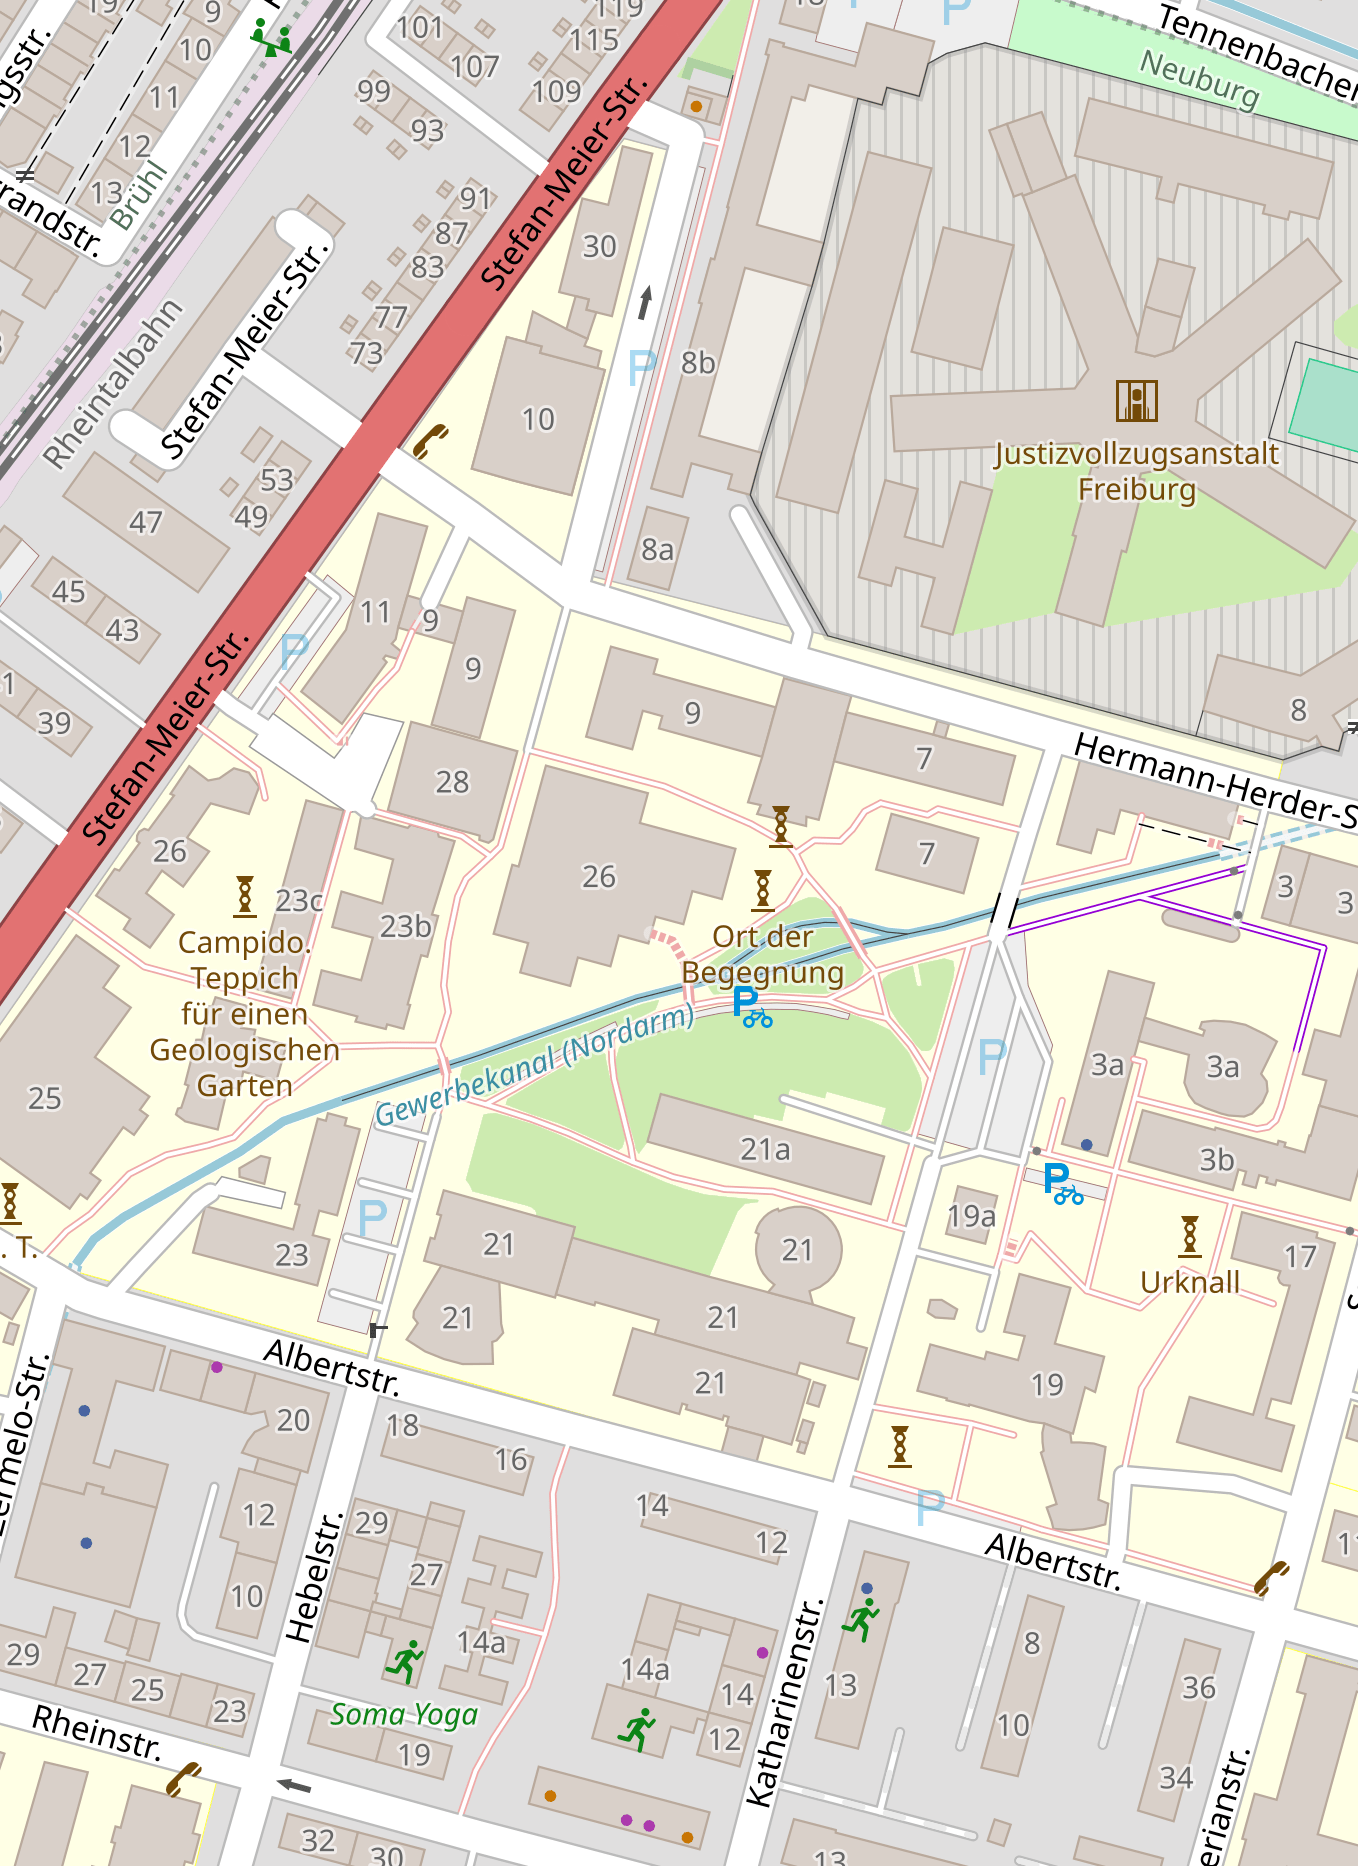
\includegraphics[width=115mm]{images-print/freiburg-campus.png}%
      };%
      % box for map key
      \fill [white] (0,39) rectangle (52,0);%
      % map key text
      \draw (8,8) node [anchor=south west, align=left] {%
        \begin{minipage}{47mm}%
          \small
          1 Hörsaal Rundbau \linebreak
          2 Ausstellung, Welcome Desk \linebreak
          3 Hörsaal Anatomie \linebreak
          4 Hörsaal Weismannhaus \linebreak
          5 Workshopräume \linebreak
          6 Hermann-Herder-Str. 9, R\,00\,020\linebreak
          7 Albertstr. 21, R\,00\,004\linebreak
          8 Mensa
        \end{minipage}%
      };
      % circles with numbers
      \node (1) at (67.00,49.50) [] {}; % HS Rundbau
      \node (1label) at (1) [fill=geoblau, draw=black, inner sep=0.3mm, circle] {1}; % HS Rundbau
      \node (2) at (64.00,40.00) [] {}; % Chemie-Hochhaus
      \node (2label) at (2) [fill=white, draw=black, inner sep=0.3mm, circle] {2}; % Chemie-Hochhaus
      \node (3) at (91.50,33.50) [] {}; % HS Anatomie
      \node (3label) at (3) [fill=hellgelb, draw=black, inner sep=0.3mm, circle] {3}; % HS Anatomie
      \node (4) at (69.50,59.00) [] {}; % HS Weismannhaus
      \node (4label) at (4) [fill=hellgruen, draw=black, inner sep=0.3mm, circle] {4}; % HS Weismannhaus
      \node (5) at (45.00,119.50) [] {}; % Workshopräume
      \node (5label) at (5) [fill=dezentrot, draw=black, inner sep=0.3mm, circle] {5}; % Workshopräume
      \node (6) at (55.00,98.50) [] {}; % BoF 1
      \node (6label) at (6) [fill=white, draw=black, inner sep=0.3mm, circle] {6}; % BoF 2
      \node (7) at (55.00,49.00) [] {}; % BoF 2
      \node (7label) at (7) [fill=white, draw=black, inner sep=0.3mm, circle] {7}; % BoF 2
      \node (8) at (51.00,87.00) [] {}; % Mensa
      \node (8label) at (8) [fill=white, draw=black, inner sep=0.3mm, circle] {8}; % Mensa
    \end{tikzpicture}%
  }%
]{campuskarte}
\newpairofpagestyles[]{page-campuskarte}{}
\AddLayersAtBeginOfPageStyle{page-campuskarte}{campuskarte}
\AddLayersAtBeginOfPageStyle{page-campuskarte}{cropmarksplain}


\begin{document}
 
\pagestyle{cropmarksstyle}
\begin{titlepage}
%  \thispagestyle{titlestyle}
  \null
\end{titlepage}
\pagestyle{cropmarksstyle}

\section*{Inhalt}
\label{contents}
\newlength\contentspace
\setlength\contentspace{0.2em}

\vspace*{\contentspace}%
\noindent Abendveranstaltung, Exkursionen, Rahmenprogramm  \dotfill \pageref{schwaetzli}

\vspace*{\contentspace}%
\noindent Workshops am Mittwoch \dotfill \pageref{mittwoch-workshops}

\vspace*{\contentspace}%
\noindent Workshops am Donnerstag \dotfill \pageref{donnerstag-workshops}

\vspace*{\contentspace}%
\noindent Workshops am Freitag \dotfill \pageref{freitag-workshops}

\vspace*{\contentspace}%
\noindent Vorträge am Mittwoch \dotfill \pageref{mittwoch}

\vspace*{\contentspace}%
\noindent Vorträge am Donnerstag \dotfill \pageref{donnerstag}

\vspace*{\contentspace}%
\noindent Vorträge am Freitag \dotfill \pageref{freitag}

\vspace*{\contentspace}%
\noindent OpenStreetMap-Samstag \dotfill \pageref{samstag}

\vspace*{\contentspace}%
\noindent Impressum \dotfill \pageref{impressum}

\vspace*{\contentspace}%
\noindent Campusplan und Raumpläne \dotfill \pageref{kartenseiten}

\justifying

\newpage

\newpage
\section*{Willkommen zur FOSSGIS-Konferenz 2023 in Berlin!}\label{welcome}
Die Abkürzung { FOSSGIS} steht für {\bfseries f}reie und {\bfseries O}pen"={\bfseries S}ource"={\bfseries S}oftware für {\bfseries G}eo{\bfseries i}nformations{\bfseries s}ysteme.
Die FOSSGIS-Konferenz 2023 wird vom gemeinnützigen FOSSGIS e.V., der
OpenStreetMap"=Community und der Humboldt-Universität zu Berlin
veranstaltet.
Ziel der jährlich stattfindenden Konferenz ist die Verbreitung von freier,
quelloffener Software für Geoinformationssysteme. In den nächsten vier Tagen
haben Sie die Gelegenheit, sich mit Entwicklern und anderen Anwendern
auszutauschen und \mbox{neueste} Informationen zu Anwendungen und
Arbeitsmöglichkeiten zu erhalten.

\section*{Anwender- und Expert:inentreffen, Birds of a Feather}
Die FOSSGIS-Konferenz ist eine Communityveranstaltung.
Die gesamte Konferenz über stehen zwei Räume für Anwender- und Expert:innentreffen oder spontan organisierte
Treffen Gleichgesinnter (Birds of a Feather), u.\,ä.
zur Verfügung. Eigene Sessions können Sie an der Pinnwand beim
Welcome Desk selbst eintragen.

\section*{Abendveranstaltung am Mittwoch}\label{schwaetzli}
Traditionell findet am ersten Abend der FOSSGIS-Konferenz die
Abendveranstaltung statt, auch Social Event genannt. Der Eintritt
ist im FOSSGIS-Konferenz-Ticket enthalten. Eine Anmeldung ist erforderlich.
Die Abendveranstaltung wird am Konferenzstandort im Erwin-Schrödinger-Zentrum
ab {\bfseries 18.30 bis 22.00 Uhr} stattfinden.

\section*{Exkursionen}
\subsection*{Kartenabteilung der Staatsbibliothek zu Berlin}
Von den Sektionskarten von Balbi und der Preußischen Uraufnahme zu digitalen Kartendaten.
Am {\bfseries Freitagnachmittag} und {\bfseries Samstagvormittag} werden Führungen durch die Karten\-abteilung der Staatsbibliothek zu Berlin im Haus Unter den Linden angeboten. Wer noch nicht angemeldet ist, wende sich bitte an den Helpdesk.
\pagebreak

\subsection*{Campus Adlershof/WISTA-Gelände}
Die FOSSGIS 2023 findet auf dem Gelände des Wissenschafts- und Wirtschaftsstandort Adlershof (WISTA) statt. Dort existieren noch mehrere technische Denkmale, wie beispielsweise der Trudelturm, die an den Beginn der Luftfahrtindustrie auf dem Campus erinnern. Zu sehen sind aber auch moderne Forschungseinrichtungen, Gründer- und Technologiezentren, die auf die heutige Entwicklung als Zukunftsort für Forschung und Innovation verweisen. In einer kleinen, etwa 60-minütigen Führung können wir sowohl dieser Geschichte als auch den neuen Trends nachstöbern und mehr über den Standort Adlershof erfahren.
Die Exkursion startet am {\bfseries Freitag} um {\bfseries 16:30 Uhr} (nach dem Sektempfang) vor dem Haupteingang des Erwin-Schrödinger-Zentrums. Wer noch nicht angemeldet ist, wende sich bitte an den Helpdesk.

\subsection*{Mapathon mit Ärzte ohne Grenzen}
Ärzte ohne Grenzen lädt im Rahmen der FOSSGIS Konferenz 2023 zu einem Mapathon ein. Die Initiative hat das Ziel die Erstellung und Vervollständigung von Kartenmaterial zu unterstützen, welches die Hilfe für Menschen in Krisengebieten erleichtern kann. Es wird eine Einführung geben. Weitere Informationen sind hier zu finden. FOSSGIS-Teilnehmende sind eingeladen, mitzumachen, auch wenn sie noch nie gemappt haben.
Termine: {\bfseries Freitag, 17.00 bis 20.00 Uhr} und {\bfseries Samstag, 11.00 bis 14.00 Uhr}. Bitte melden Sie sich über den Anmeldelink auf der Konferenzwebseite an.

\section*{Rahmenprogramm am Donnerstag}
\subsection*{Gruppenfoto}
Auch in diesem Jahr wollen wir uns das Gruppenfoto nicht entgehen lassen und laden Sie ein am {\bfseries Donnerstag} in der {\bfseries Nachmittagspause} zum gemeinsamen Gruppenfoto am Haupteingang des Erwin-Schrödinger-Zentrums ein.

\subsection*{Treffen der Freiberufler}
Am {\bfseries Donnerstag} werden sich um {\bfseries 17.45 Uhr} die Freiberufler aus dem FOSSGIS-Bereich im Seminarraum 1'306 zum gemeinsamen Austausch treffen.

\subsection*{Mitgliederversammlung des FOSSGIS e.\,V.}
Am {\bfseries Donnerstag} sind alle Mitglieder und Gäste ab {\bfseries 18.00 Uhr} herzlich eingeladen, an der Mitgliederversammlung teilzunehmen und sich zu beteiligen. Der FOSSGIS e.\,V. lädt zum Diskutieren, Kennenlernen, Abstimmen und zu Neuwahlen ein. Es wird Getränke geben und es Pizza für alle bestellt werden. Der Verein freut sich über zahlreiches Erscheinen.

\section*{Rahmenprogramm am Freitag}
\subsection*{Jeopardy-Quiz}
Am {\bfseries Freitag} gibt es vor dem Abschluss des reguläres Konferenzprogramms um {\bfseries 14.30 Uhr} das nunmehr legendäre und sehr humorvolle Quiz in Form des FOSSGIS-Jeopardy mit Hannes und Tobia.

\subsection*{Sektempfang am FOSSGIS-Stand}
Alle Mitglieder des FOSSGIS-Vereins, Freunde und Interessierte sind am {\bfseries Freitag} ab {\bfseries 16.00 Uhr} herzlich zum Sektempfang zum Ausklang der FOSSGIS 2023 am FOSSGIS-Vereins-Stand eingeladen.

\subsection*{OSM-Event am Freitagabend}
Für alle, die am {\bfseries Freitagabend} noch in der Stadt sind und/oder am OSM-Event teilnehmen möchten, wird ein gemeinsamer Treffpunkt zur Abendgestaltung bekannt gegeben.

\newpage
\label{platinsposoren}
\section*{Platinsponsor und Aussteller}
\begin{center}
  
\includegraphics[width=0.7\textwidth]{001_camptocamp_logo.png}
\end{center}
Camptocamp gehört zu den führenden Dienstleistern im Bereich Open-Source-GIS und ist in vielen unterschiedlichen Open-Source-Communitys stark engagiert.

Unsere Dienstleistungen stützen sich auf 20 Jahre Erfahrung in der Umsetzung von innovativen GIS-Lösungen für Behörden und Unternehmen und erlauben einen hochwertigen und individuellen Service. Das Besondere an Camptocamp sind die hochqualifizierten Mitarbeiter und ihr großes Engagement im "`Ökosystem"' der eingesetzten Open-Source-Software-Lösungen, indem sehr enge Beziehungen zu den Herstellern der jeweiligen Produkte gepflegt werden.

Um die oft anspruchsvollen Projekte umzusetzen, erstellt Camptocamp individuelle Lösungen, die auf den am besten geeigneten und fortschrittlichsten Open-Source-Technologien basieren. Camptcamp ist in München, Lausanne, Olten, Paris und Chambéry vertreten und bietet neben Lösungen im GIS-Bereich auch eine große Expertise im den Bereichen ERP (Enterprise-Resource-Planning) und IT-Infrastruktur-Lösungen.

\newpage
\section*{Platinsponsor und Aussteller}

\vspace{-0.2cm}
\centerline{
\includegraphics[width=0.7\textwidth]{002_WhereGroup.jpg}}
\noindent
Die WhereGroup ist eines der größten Open-Source-Software\-häuser der GEO-IT-Branche in Deutschland. Wir managen zahlreiche komplexe GIS-Projekte unterschiedlichster Art. Als mittelständisches Unternehmen mit über 40 Mitarbeiter*innen an vier Standorten arbeiten wir innovativ und haben dennoch die Bodenhaftung nicht verloren.

Wir bieten Ihnen kompetente Unterstützung in den Bereichen Geographische Informationssysteme (GIS), Web-GIS, Datenbanken, Standards, Interoperabilität und System-Integration. Angefangen bei der Beratung, Konzeption und Entwicklung bis hin zum Betrieb dynamischer Kartenanwendungen im Intra- und Internet.

Grundlage unseres Schaffens ist der Open-Source-Gedanke. Als Teil einer starken Community, mit der wir in engem Austausch stehen, engagieren wir uns aus Überzeugung im FOSSGIS e.\,V., im QGIS-DE e.\,V. und bei der OSGeo. Wir sind aus voller Überzeugung auf Open-Source-Entwicklungen spezialisiert und integrieren professionelle freie Software nahtlos in proprietäre Systeme.

Wir implementieren Lösungen für den Mittelstand, die Industrie und auf allen Ebenen der öffentlichen Verwaltung, beraten und begleiten bei Planung, Migration und Einführung von raumbezogenen Informationssystemen.

Dabei reicht das Spektrum unserer Projekte von Desktop-Lösungen über Geoportalen und kartenbasierter Datenverwaltung bis hin zu hochverfügbaren Anwendungen für die freie Wirtschaft und die öffentliche Verwaltung.

Unser Schulungsinstitut, die FOSS Academy, bietet außerdem praxisorientierte Schulungen zum Thema "`GIS mit Open-Source-Software"' an.

Mehr zur WhereGroup unter www.wheregroup.com und www.foss-academy.com.
\normalsize

\newpage
\section*{Platinsponsor und Aussteller}

\vspace{-0.5cm}
\centerline{
\includegraphics[width=0.5\textwidth]{003_hu_siegel-kombi_rgb.png}}
Die Humboldt-Universität zu Berlin, gegründet 1810, ist die älteste Hochschule in Berlin
und eine der renommiertesten Universitäten weltweit. Das Lehr- und Forschungsangebot der HU umfasst heute alle grundlegenden
Wissenschaftsdisziplinen der Geistes-, Sozial- und Kulturwissenschaften, der Rechtswissenschaften, der Lebenswissenschaften, der Mathematik und Naturwissenschaften, der Medizin, der Agrarwissenschaften und der Nachhaltigkeits- und Antikeforschung. Aktuell studieren an der Humboldt-Universität fast 37.000 junge Menschen aus über 100 Ländern in 171 Bachelor- und Masterstudiengängen betreut von über 400 Professor:innen. Zirka 34 Prozent der wissenschaftlichen Mitarbeiter:innen kommen aus anderen Ländern.Aufgrund zahlreicher Projekte der Spitzenforschung und renommierter internationaler Netzwerke ist die Humboldt-Universität eine der bedeutendsten Universitäten im deutschsprachigen Raum. Bei der Exzellenzstrategie 2019 wurde sie gemeinsam mit den Partner:innen der Berlin University Alliance als Exzellenzverbund ausgezeichnet. Zuvor gehörte sie seit 2012 zu einer der elf deutschen Exzellenzuniversitäten. Die HU verbindet Forschungsexzellenz mit innovativer Nachwuchsförderung. Im Fokus der Lehre stehen forschendes Lernen, Interdisziplinarität und Internationalisierung.

\newpage
\section*{Platinsponsor und Aussteller}

\vspace{-0.5cm}
\centerline{
\includegraphics[width=0.9\textwidth]{004_TSB_quer.png}}
Die Technologiestiftung Berlin ist eine unabhängige und gemeinnützige Stiftung. Wir arbeiten für ein lebenswertes, smartes Berlin – und eine lebendige, transparente Stadtgesellschaft, die alle am digitalen Wandel teilhaben lässt. Mit digitalen Tools und smarten Lösungen tragen wir aktiv dazu bei, dass Berlin offen, nachhaltig und effizient wird. Viele unserer Projekte sind Leuchttürme, die beispielhaft die Chancen der Digitalisierung zeigen und Berlin über die Stadtgrenzen hinaus profilieren.

Open Data und Open Source gehören zu unserer DNA. Gemeinsam mit Stadtgesellschaft, Verwaltung, Wissenschaft und Unternehmen nutzen wir das Potenzial offener Daten und Anwendungen, um Transparenz zu schaffen, Teilhabe zu ermöglichen und innovative Lösungen zu fördern. Und das in ganz unterschiedlichen Bereichen: Mit der Senatsverwaltung für Inneres, Digitalisierung und Sport bieten wir die Open Data Informationsstelle an. Sie unterstützt die Berliner Verwaltung bei der Bereitstellung offener Daten und entwickelt darauf basierend eigene Anwendungen wie die Visualisierung der Berliner Haushaltsdaten oder das Organigramm-Tool. Im Projekt kulturdaten.berlin schaffen wir die erste offene, digitale Infrastruktur für Kulturschaffende und -institutionen in Berlin, gefördert durch die Senatsverwaltung für Kultur und Europa. Und die Open-Map-Anwendung Gieß den Kiez vom CityLAB Berlin ermöglicht Bürger:innen die Pflege von über 800.000 Stadtbäumen.

Auf der FOSSGIS freuen wir uns auf den gemeinsamen Austausch und neue Impulse zu offenen Daten sowie Datenbank- und OpenStreetMap-Anwendungen!
\normalsize

\newpage
\section*{Goldponsor und Aussteller}

\centerline{
\includegraphics[width=0.9\textwidth]{101_BKG_Logo_RGB.png}}

Das Bundesamt für Kartographie und Geodäsie (BKG) ist eine Behörde im Geschäftsbereich des Bundesministeriums des Innern und für Heimat (BMI). Es fungiert als zentraler Dienstleister des Bundes und Kompetenzzentrum für Geoinformation und geodätische Referenzsysteme. Das BKG befasst sich mit der Beobachtung sowie der Datenhaltung bis hin zur Analyse, Kombination und Bereitstellung von Geodaten. Das BKG ermöglicht aufgrund der zentralen Geodatenbereitstellung eine optimale und wirtschaftliche Geodatennutzung im Bundesbereich.

Das BKG setzt sich für eine offene Datenpolitik ein, wodurch die Verbreitung von Open Data gefördert wird. Dies schließt die Beratung anderer Bundesbehörden beim Umgang mit OSM-Daten ein. Die Nutzung, Entwicklung und Verbreitung der Nutzung freier Software liegen ebenfalls im Bereich der Aktivitäten.

Von der Arbeit des BKG profitieren insbesondere Bundeseinrichtungen, die öffentliche Verwaltung, Wirtschaft, Wissenschaft – und fast jeder Bürger in Deutschland. Experten aus den verschiedensten Bereichen wie Verkehr, Katastrophenvorsorge, Innere Sicherheit, Energie und Umwelt verwenden Geodaten, Landkarten, Referenzsysteme und Informationsdienste des BKG für ihre Pläne und Untersuchungen. Das BKG unterhält ein Dienstleistungszentrum in Leipzig sowie geodätische Observatorien im In- und Ausland.

\newpage
\section*{Goldponsor und Aussteller}
\begin{center}
  
\includegraphics[width=0.8\textwidth]{102_Logo_QFieldCloud-by-OpenGIS_transparent.png}
\end{center}
Wir planen und entwickeln personalisierte Open Source GIS Lösungen als Desktop-, Web- oder Mobilapplikationen für Ingenieurbüros, Organisationen und den öffentlichen Sektor – kosteneffizient, massgeschneidert und von A bis Z. Mit Open Source Technologie-Erfahrung, POSTGIS Expertise und QGIS und QField Entwicklerwissen finden wir elegante Lösungen auch für komplexe Aufgaben. Darauf geben wir Ihnen unser Schweizer GeoNinja-Ehrenwort - oder einen Support Vertrag mit SLA.

Aber nicht nur wir sind von uns überzeugt. Viel wichtiger, auch die Deutsche Bahn, das Bundesamt für Umwelt, mehrere Kantone und weitere Auftraggeber sind sich einig: OPENGIS.ch ist der ideale Partner, wenn es um Open Source GIS Projekte geht.

QFieldCloud ergänzt die mobile Applikation QField für die Synchronisierung der erfassten Daten und erleichtert die Zusammenarbeit von mehreren Personen oder Teams im Feld. Nutzer und Rollen werden klar definiert, Änderungen können nachverfolgt und erfasste Daten einfach über die Cloud synchronisiert werden.


\newpage
\section*{Workshops am Mittwoch}
\label{mittwoch-workshops}
\newSmallTimeslot{10:30}
% Hack, um Einrücken des ersten Workshops wieder rückgängig zu machen
\RaggedRight
% time: Wednesday 10:30
% URL: https://pretalx.com/fossgis2020/talk/VCJD7E/
\noindent\workshop{GeoPython mit dem Jupyter Notebook~--\linebreak Rasterdaten}{Christian Strobl}{SR R-100}
\workshopspace

%%%%%%%%%%%%%%%%%%%%%%%%%%%%%%%%%%%%%%%%%%%

% time: Wednesday 10:30
% URL: https://pretalx.com/fossgis2020/talk/G7ZZ3Z/


\noindent\workshop{INSPIRE "`instant"' 2.x}{Armin Retterath}{SR R-110}
\workshopspace

%%%%%%%%%%%%%%%%%%%%%%%%%%%%%%%%%%%%%%%%%%%

% time: Wednesday 10:30
% URL: https://pretalx.com/fossgis2020/talk/3EDG7S/


\noindent\workshop{Eigene Verarbeitungswerkzeuge für QGIS\linebreak
mit Python erstellen}{Peter Gipper}{SR R-114}
\workshopspace

%%%%%%%%%%%%%%%%%%%%%%%%%%%%%%%%%%%%%%%%%%%

% time: Wednesday 15:00
% URL: https://pretalx.com/fossgis2020/talk/RERSW7/

\newSmallTimeslot{15:00}
\noindent\workshop{Grafische Prozessmodellierung mit QGIS}{Claas Leiner}{SR R-100}
\workshopspace

%%%%%%%%%%%%%%%%%%%%%%%%%%%%%%%%%%%%%%%%%%%

% time: Wednesday 15:00
% URL: https://pretalx.com/fossgis2020/talk/E8KJSG/


\noindent\workshop{Orchestrierung einer GDI über Docker}{Jan Suleiman, Daniel Koch}{SR R-110}
\workshopspace

%%%%%%%%%%%%%%%%%%%%%%%%%%%%%%%%%%%%%%%%%%%

% time: Wednesday 15:00
% URL: https://pretalx.com/fossgis2020/talk/SWV3BY/


\noindent\workshop{Einführung in OpenLayers}{Marc Jansen, Christian Mayer, Andreas Hocevar}{SR R-114}
\workshopspace

%%%%%%%%%%%%%%%%%%%%%%%%%%%%%%%%%%%%%%%%%%%

% time: Wednesday 17:00
% URL: https://pretalx.com/fossgis2020/talk/MB9ZLH/

\newSmallTimeslot{17:00}
\noindent\workshop{QGIS~3 Einsteiger-Workshop}{Otto Dassau, Tristan}{SR R-100}
\workshopspace

%%%%%%%%%%%%%%%%%%%%%%%%%%%%%%%%%%%%%%%%%%%

% time: Wednesday 17:00
% URL: https://pretalx.com/fossgis2020/talk/EJSF9F/


\noindent\workshop{SQL für Fortgeschrittene}{Felix Kunde}{SR R-110}
\workshopspace

%%%%%%%%%%%%%%%%%%%%%%%%%%%%%%%%%%%%%%%%%%%

% time: Wednesday 17:00
% URL: https://pretalx.com/fossgis2020/talk/XQ7QNS/


\noindent\workshop{Einfacher Aufbau von Web-GIS-Anwendungen mit Mapbender}{Jörg Thomsen}{SR R-114}
\workshopspace

\section*{Workshops am Donnerstag}
\label{donnerstag-workshops}
%%%%%%%%%%%%%%%%%%%%%%%%%%%%%%%%%%%%%%%%%%%

% time: Thursday 09:00
% URL: https://pretalx.com/fossgis2020/talk/HFMLCC/

\newSmallTimeslot{09:00}
\noindent\workshop{QGIS-Basics für Anfänger und Umsteiger}{Helene Kautz}{SR R-100}
\workshopspace

%%%%%%%%%%%%%%%%%%%%%%%%%%%%%%%%%%%%%%%%%%%

% time: Thursday 09:00
% URL: https://pretalx.com/fossgis2020/talk/JHQ9Q3/


\noindent\workshop{Eigene Verarbeitungswerkzeuge für QGIS\linebreak
mit Python erstellen}{Peter Gipper}{SR R-110}
\workshopspace

%%%%%%%%%%%%%%%%%%%%%%%%%%%%%%%%%%%%%%%%%%%

% time: Thursday 09:00
% URL: https://pretalx.com/fossgis2020/talk/BPWXKG/


\noindent\workshop{Einführung in GeoServer}{Daniel Koch, Hannes Blitza}{SR R-114}
\workshopspace

%%%%%%%%%%%%%%%%%%%%%%%%%%%%%%%%%%%%%%%%%%%

% time: Thursday 11:00
% URL: https://pretalx.com/fossgis2020/talk/CKSRYB/

\newSmallTimeslot{11:00}
\noindent\workshop{QGIS~-- Fortgeschrittene Datenvisualisierung mit Live-Layer-Effekten und Mischodi}{Stefan Giese}{SR R-110}
\workshopspace

%%%%%%%%%%%%%%%%%%%%%%%%%%%%%%%%%%%%%%%%%%%

% time: Thursday 11:00
% URL: https://pretalx.com/fossgis2020/talk/CBMDZY/


\noindent\workshop{Workshop Open Database License}{Falk Zscheile}{SR R-114}
\workshopspace

%%%%%%%%%%%%%%%%%%%%%%%%%%%%%%%%%%%%%%%%%%%

% time: Thursday 13:30
% URL: https://pretalx.com/fossgis2020/talk/YKAGHX/

\newSmallTimeslot{13:30}
\noindent\workshop{GeoStyler~-- Eine UI für alle* Stile}{Christian Mayer, Jan Suleiman}{SR R-100}
\workshopspace

%%%%%%%%%%%%%%%%%%%%%%%%%%%%%%%%%%%%%%%%%%%

% time: Thursday 13:30
% URL: https://pretalx.com/fossgis2020/talk/TVAGUN/


\noindent\workshop{Geodaten jonglieren mit ogr2ogr}{Claas Leiner}{SR R-110}
\workshopspace

%%%%%%%%%%%%%%%%%%%%%%%%%%%%%%%%%%%%%%%%%%%

% time: Thursday 15:30
% URL: https://pretalx.com/fossgis2020/talk/VUPGUK/

\newSmallTimeslot{15:30}
\noindent\workshop{Dateneingabeformulare gestalten mit \mbox{Qt-Designer} und Python}{Otto Dassau, Tristan}{SR R-100}
\workshopspace

%%%%%%%%%%%%%%%%%%%%%%%%%%%%%%%%%%%%%%%%%%%

% time: Thursday 15:30
% URL: https://pretalx.com/fossgis2020/talk/7RFJ9N/


\noindent\workshop{Einführung in die Verwaltung von Geodaten in der PostgreSQL-Datenbank mit PostGIS}{Astrid Emde, Lina Dillmann}{SR R-110}
\workshopspace

\section*{Workshops am Freitag}
\label{freitag-workshops}

%%%%%%%%%%%%%%%%%%%%%%%%%%%%%%%%%%%%%%%%%%%

% time: Friday 09:00
% URL: https://pretalx.com/fossgis2020/talk/RUEZJ7/

\newSmallTimeslot{09:00}
\noindent\workshop{Einführung in die Verwaltung von Geodaten in der PostgreSQL-Datenbank mit PostGIS}{Astrid Emde, Leoni Möske}{SR R-100}
\workshopspace

%%%%%%%%%%%%%%%%%%%%%%%%%%%%%%%%%%%%%%%%%%%

% time: Friday 09:00
% URL: https://pretalx.com/fossgis2020/talk/7KUG7F/


\noindent\workshop{Workshop Datenschutz und geographische Informationen}{Falk Zscheile}{SR R-110}
\workshopspace

%%%%%%%%%%%%%%%%%%%%%%%%%%%%%%%%%%%%%%%%%%%

% time: Friday 09:00
% URL: https://pretalx.com/fossgis2020/talk/CF778N/


\noindent\workshop{GRASS GIS per HTTP: actinia Geoprozessierung}{Jan Suleiman, Carmen Tawalika}{SR R-114}
\workshopspace

%%%%%%%%%%%%%%%%%%%%%%%%%%%%%%%%%%%%%%%%%%%

% time: Friday 11:00
% URL: https://pretalx.com/fossgis2020/talk/URWELU/

\newSmallTimeslot{11:00}
\noindent\workshop{QGIS-Ausdruckskseditor und Geometrie-Generator}{Stefan Giese}{SR R-100}
\workshopspace

%%%%%%%%%%%%%%%%%%%%%%%%%%%%%%%%%%%%%%%%%%%

% time: Friday 11:00
% URL: https://pretalx.com/fossgis2020/talk/7DJMEJ/


\noindent\workshop{GeoServer-Vertiefung}{Daniel Koch, Hannes Blitza}{SR R-110}
\workshopspace

%%%%%%%%%%%%%%%%%%%%%%%%%%%%%%%%%%%%%%%%%%%

% time: Friday 11:00
% URL: https://pretalx.com/fossgis2020/talk/DMVYS9/


\noindent\workshop{Bessere Höhenlinien aus Geländemodelle erstellen}{Mathias Gröbe}{SR R-114}
\workshopspace

%%%%%%%%%%%%%%%%%%%%%%%%%%%%%%%%%%%%%%%%%%%
\justifying
\sponsorBoxA{101-terrestris.pdf}{0.42\textwidth}{5}{%
\textbf{Silbersponsor, Aussteller}\\
\noindent terrestris ist Dienstleister für maßgeschneiderte Geoinformations"=Lösungen mit Freier und Open-Source-Software.
Wir entwickeln Lösungen, die den tatsächlichen Anforderungen unserer Kunden entsprechen. Dies ist nach unserem eigenen Verständnis auch Grundlage unserer fairen, transparenten und häufig langfristigen Kundenbeziehungen.
Dabei decken wir das gesamte Spektrum von Beratung, Konzeptionierung, Entwicklung bis hin zu Wartung \& Support an.
Unser Leistungsspektrum erstreckt sich auf folgende Bereiche:

Geoportale \& Stadtplandienste
Fachanwendungen für unterschiedlichste Branchen
Visualisierung von 3D-Daten im Browser
Nutzung von OpenStreetMap (z.B. OSM WMS)
QGIS
}


\newpage
\renewcommand{\arraystretch}{1.4}
\section*{Vorträge am Mittwoch}\label{mittwoch}
\renewcommand{\conferenceDay}{\mittwoch}
\setPageBackground
\noindent\begin{tabular}{Z{0.85cm}Z{6.85cm}}
  & \multicolumn{1}{c}{\cellcolor{hellgelb} Anatomie}
  \tabularnewline
  10:30
  \talk{Die Welt als runde Sache auf der ebenen Karte}{Wolfgang Hinsch}
  \tabularnewline
  11:00
  \talk{Ehrenamt im FOSSGIS e.V.}{Hanna Krüger}
  \tabularnewline
  11:25
  \talk{Was ist Open Source?}{Marco Lechner}
  \tabularnewline
  11:40
  \talk{Was ist OpenStreetMap?}{Thomas Skowron}
  \tabularnewline
  \rowcolor{commongray}
  12:00 & \multicolumn{1}{c}{%
    \parbox[c]{24pt}{%
      
\includegraphics[height=10pt]{restaurant}%
    }
    Mittagspause
  } \tabularnewline
\end{tabular}

\vspace{0.5\baselineskip}
\noindent\begin{tabular}{Z{0.85cm}Z{6.85cm}}
  & \multicolumn{1}{c}{\cellcolor{geoblau} Rundbau} \tabularnewline
  13:00
  \talk{Eröffnungs\-veranstaltung}{}
  \tabularnewline
  13:45
  \talk{\emph{Keynote} Pilgerstab in einer Hand, Brecheisen in der anderen}{Guillaume Rischard}
  \tabularnewline
  \rowcolor{commongray}
  14:30 & \multicolumn{1}{c}{%
    \parbox[c]{24pt}{%
      
\includegraphics[height=10pt]{cafe}%
    }
    Kaffeepause} \tabularnewline
\end{tabular}
\newpage

\vspace{0.5\baselineskip}
\enlargethispage{1.0\baselineskip}
\renewcommand{\arraystretch}{1.3}
\noindent\begin{tabular}{lZ{2.0cm}Z{2.0cm}Z{2.0cm}}
  & \multicolumn{1}{c}{\cellcolor{geoblau} Rundbau}
  & \multicolumn{1}{c}{\cellcolor{hellgelb} Anatomie}
  & \multicolumn{1}{c}{\cellcolor{hellgruen} Weismannhaus}
  \tabularnewline
  15:00
  \talk{Von ArcGis nach QGIS}{Peter Heidelbach}
  \talk{2700 interaktive thematische Karten~-- ein Fall für Vector Tiles!}{Pirmin Kalberer}
  \talk{%Weniger ist mehr~-- Zur
  Auswahl darzustellender Elemente in der digitalen Kartographie}{Christoph \mbox{Hormann}}
  \tabularnewline
  15:30
  \talk{QGIS im Produktivbetrieb}{Thomas Baumann}
  \talk{Kartenherstellung zwischen Lizenzen, Daten, Programmcode und Darstellung}{Falk Zscheile}
  \talk{Umgang mit % vorhandenen und
  fehlenden Relevanzinformationen in OSM-Kartenstilen}{Michael \mbox{Reichert}}
  \tabularnewline
  16:00
  \talk{WebGIS kleiner Gemeinden mit QGIS-Server und Lizmap}{Günter Wagner}
  \talk{FAIRe Daten und FAIRe Software in der Biodiversitätsforschung}{Bernhard Seeger}
  \talk{Reliefdarstellung mit Höhenlinien}{Mathias Gröbe}
  \tabularnewline
\end{tabular}
\newpage
  
\begin{center}
  \renewcommand{\arraystretch}{1.3}
  \noindent\begin{tabular}{lZ{2.0cm}Z{2.0cm}Z{2.0cm}}
    & \multicolumn{1}{c}{\cellcolor{geoblau} S239}
    & \multicolumn{1}{c}{\cellcolor{hellgelb} Z211}
    & \multicolumn{1}{c}{\cellcolor{hellgruen} Z254}
    \tabularnewline
    \rowcolor{commongray}
    16:30 & \multicolumn{3}{c}{%
    \parbox[c]{24pt}{%
      
\includegraphics[height=10pt]{cafe}%
    }
    Kaffeepause} \tabularnewline
    17:00
    \talk{OSM-Daten in QGIS nutzen}{Astrid Emde}
    \talk{Ein einheitlicher Frontend"=Ansatz, um mehrere Routing"=Lösungen im Web-GIS zu nutzen}{Robert Klemm}
    \talk{GeoPortal Koblenz~-- digital, vielschichtig, maßgebend}{Andreas Weckbecker, Christine Dolezich}
    \tabularnewline
    17:30
    & \emph{Bitte Aushang beachten}
    \longTalk{2}{\emph{Demosession} Einführung zu GDAL/OGR: Geodaten mit der Kommandozeile verarbeiten}{Jakob Miksch}
    \talk{Der ÖREB-Kataster~-- eine Ode an offene Standards und Software}{Stefan Ziegler}
    \tabularnewline
    18:00
    \talk{Lightning Talks}{}
    &
    \talk{GeoPortal.rlp unchained}{Armin Retterath}
    \tabularnewline
    \rowcolor{commongray}
    19:00 &
    \multicolumn{3}{c}{%
      \parbox[c]{24pt}{%
        
\includegraphics[height=10pt]{restaurant}%
      }
      Schwätzli uffem Campus (siehe Seite \pageref{schwaetzli})
    }
    \tabularnewline
  \end{tabular}
\end{center}
\renewcommand{\arraystretch}{1.0}


% time: Wednesday 10:30
% URL: https://pretalx.com/fossgis2020/talk/JV7GRQ/

%
\newTimeslot{10:30}
\noindent\abstractHSAnatomie{%
  Wolfgang Hinsch%
}{%
  Die Welt als runde Sache auf der ebenen Karte%
}{%
}{%
  Es ist nicht möglich, die Erde verzerrungsfrei auf einer Karte darzustellen. Es wird gezeigt, mit
  welchem Abbildungssystem OSM arbeitet, welche Vor- und Nachteile es hat, und eine Auswahl
  relevanter alternativer Koordinatenbezugssysteme aufgezeigt. Dabei werden Begriffe wie
  Referenzellipsoid, Geoid, EPSG, WGS84, NHN etc. vorgestellt.%
}%


%%%%%%%%%%%%%%%%%%%%%%%%%%%%%%%%%%%%%%%%%%%

% time: Wednesday 11:00
% URL: https://pretalx.com/fossgis2020/talk/QMK3JN/

%
\newTimeslot{11:00}
\noindent\abstractHSAnatomie{%
  Hanna Krüger%
}{%
  Ehrenamt im FOSSGIS e.V.%
}{%
}{%
  Was ist eigentlich der FOSSGIS e.V. und was ist sein Ziel, wie funktioniert er und wie sieht das
  Vereinsleben aus?%
}%


%%%%%%%%%%%%%%%%%%%%%%%%%%%%%%%%%%%%%%%%%%%

% time: Wednesday 11:25
% URL: https://pretalx.com/fossgis2020/talk/EZAY3D/

%
\newTimeslot{11:25}
\noindent\abstractHSAnatomie{%
  Marco Lechner%
}{%
  Was ist Open Source?%
}{%
}{%
  Der Vortrag stellt die Geschichte der Entwicklung von Open Source vor und geht auf wichtige
  Grundlagen ein.
  Ziel des FOSSGIS e.V. und der OSGeo ist die Förderung und Verbreitung freier Geographischer
  Informationssysteme (GIS) im Sinne Freier Software und Freier Geodaten. Dazu zählen auch
  Erstinformation und Klarstellung von typischen Fehlinformationen über Open Source und Freie
  Software, die sich über die Jahre festgesetzt haben.%
}%


%%%%%%%%%%%%%%%%%%%%%%%%%%%%%%%%%%%%%%%%%%%

% time: Wednesday 11:40
% URL: https://pretalx.com/fossgis2020/talk/UEWFWR/

%
\newTimeslot{11:40}
\noindent\abstractHSAnatomie{%
  Thomas Skowron%
}{%
  Was ist OpenStreetMap?%
}{%
}{%
  Was ist OpenStreetMap? Die Enstehung, die heutige Bedeutung und die vielfältigen Nutzungsmöglichkeiten der offenen Weltkarte OpenStreetMap werden vorgestellt. Es werden Möglichkeiten zur Mitwirkung präsentiert.%
}%

%%%%%%%%%%%%%%%%%%%%%%%%%%%%%%%%%%%%%%%%%%%

% time: Wednesday 13:00
% URL: https://pretalx.com/fossgis2020/talk/TDNXQF/

%
\newTimeslot{13:00}
\noindent\abstractHSRundbau{%
}{%
  Eröffnung%
}{%
}{%
  Feierliche Eröffnung der Konferenz durch Vertreter des FOSSGIS e.V. mit wichtigen Hinweisen
  zu Ablauf und Organisation.%
}%


%%%%%%%%%%%%%%%%%%%%%%%%%%%%%%%%%%%%%%%%%%%

% time: Wednesday 13:45
% URL: https://pretalx.com/fossgis2020/talk/HEE3SU/

%
\newTimeslot{13:45}
\noindent\abstractHSRundbau{%
  Guillaume Rischard%
}{%
  Wie man offene Geodaten bekommt, jetzt!%
}{%
 Meine Erfahrung in Luxemburg, in der EU und au{\ss}erhalb%
}{%
}%


%%%%%%%%%%%%%%%%%%%%%%%%%%%%%%%%%%%%%%%%%%%

% time: Wednesday 15:00
% URL: https://pretalx.com/fossgis2020/talk/GPMCKV/

%
\newTimeslot{15:00}
\noindent\abstractHSAnatomie{%
  Pirmin Kalberer%
}{%
  2700 interaktive thematische Karten~-- Ein Fall für Vektortiles!%
}{%
}{%
  Die Webkarten des neuen Vogelatlas der Schweizer Vogelwarte bieten dank Vektortile-Technologie
  hohe Interaktivität bei geringem Resourcenbedarf. Der Vortrag zeigt die technischen Hintegründe,
  aber auch viele Karten!%
}%


%%%%%%%%%%%%%%%%%%%%%%%%%%%%%%%%%%%%%%%%%%%

% time: Wednesday 15:00
% URL: https://pretalx.com/fossgis2020/talk/ZFQNNN/

%

\noindent\abstractHSRundbau{%
  Peter Heidelbach%
}{%
  Von ArcGis nach QGIS%
}{%
}{%
  Für die Konvertierung von ArcGIS-Projekten in QGIS-Projekte gibt es derzeit verschiedene Ansätze.
  Die australische Firma North Road entwicklet zur Zeit ein Tool zum Reverse-Engineering der
  Binärdateien. GeoCats Bridge priorisiert dagegen den Export der ArcGIS-Layer als Web-Services. An
  einer nativen Toolbox arbeitet die WhereGroup, welche Projektdaten als QGIS-XML exportiert. Der
  Vortrag beschreibt die unterschiedlichen Vorgehensweisen und stellt Vor- und Nachteile der einzelnen
  Verfahren gegenüber.%
}%


%%%%%%%%%%%%%%%%%%%%%%%%%%%%%%%%%%%%%%%%%%%

% time: Wednesday 15:00
% URL: https://pretalx.com/fossgis2020/talk/YQGPNJ/

%

\noindent\abstractWeismannhaus{%
  Christoph Hormann%
}{%
  Weniger ist mehr~-- zur Auswahl darzustellender Elemente in der digitalen Kartographie%
}{%
}{%
  Die Auswahl von dem, was man in einer Karte darstellt, ist von entscheidender Bedeutung für deren
  Lesbarkeit.  In Karten auf Grundlage von OpenStreetMap-Daten wird diese Auswahl für viele wichtige
  Elemente durch subjektive Klassifizierungen oder die Größe subjektiver Beschriftungs-Geometrien
  vorgenommen, welche eigentlich in OpenStreetMap nichts zu tun haben.  Dieser Vortrag gibt einen
  Überblick über Ansätze zur Bewertung der Bedeutung von Objekten für den Zweck der Auswahl bei der
  Darstellung.%
}%


%%%%%%%%%%%%%%%%%%%%%%%%%%%%%%%%%%%%%%%%%%%

% time: Wednesday 15:30
% URL: https://pretalx.com/fossgis2020/talk/MYTFXF/

%
\newTimeslot{15:30}
\noindent\abstractHSAnatomie{%
  Falk Zscheile%
}{%
  Kartenherstellung zwischen Lizenzen, Daten, Programmcode und Darstellung%
}{%
}{%
  Das Urheberrecht schützt sowohl die persönlich geistige Schöpfung (Kreativität) von Personen als
  auch Datenbanken. Der Vortrag untersucht Fragen, die sich stellen, wenn virale Lizenzen (Copyleft)
  von Software, Darstellungsregeln (rendering rules)  und Datenbank (z.B. ODbL) im GIS oder Renderer
  zusammentreffen.%
}%


%%%%%%%%%%%%%%%%%%%%%%%%%%%%%%%%%%%%%%%%%%%

% time: Wednesday 15:30
% URL: https://pretalx.com/fossgis2020/talk/7BCWHD/

%

\noindent\abstractHSRundbau{%
  Thomas Baumann%
}{%
  QGIS im Produktivbetrieb%
}{%
Erfahrungsbericht zur Einführung von QGIS als\\ professionelles Planungswerkzeug%
}{%
  Seit Anfang 2016 habe ich bei einem mittelständischen Unternehmen QGIS als professionelles GIS mit
  Schwerpunkt Planung im Bereich des Breitbandausbaus eingeführt.
 In diesem Vortrag berichte ich über den Weg vom anfänglichen „fear, uncertainty, and
  doubt“ -Phänomen über erste Teilerfolge hin zu Akzeptanz von QGIS als etabliertes Werkzeug zur
  Unterstützung der Planer.
 Beleuchtet werden soll auch die technische Umsetzung zur Bereitstellung von QGIS im
  professionellen Umfeld.%
}%


%%%%%%%%%%%%%%%%%%%%%%%%%%%%%%%%%%%%%%%%%%%

% time: Wednesday 15:30
% URL: https://pretalx.com/fossgis2020/talk/S8HCFT/

%

\noindent\abstractWeismannhaus{%
  Michael Reichert%
}{%
  Umgang mit vorhandenen und fehlenden Relevanzinformationen in OpenStreetMap-Kartenstilen%
}{%
}{%
  Bei bestimmten Featureklassen ist auch in der automatisierten Kartographie die Trennung von
  wichtigen und weniger wichtigen Features von Bedeutung. OpenStreetMap-Daten enthalten Information
  über die Relevanz eines Objekts nur in bestimmten Fällen.
  Der Vortrag stellt vor, wie verschiedene OSM-Open-Source-Kartenstile vorhandenen
  Relevanzinformationen nutzen. Anschließend wird präsentiert, wie der
  OpenRailwayMap-Infra\-strukturstil Routenrelationen zur Bewertung von Haltestellen verwendet.%
}%


%%%%%%%%%%%%%%%%%%%%%%%%%%%%%%%%%%%%%%%%%%%

% time: Wednesday 16:00
% URL: https://pretalx.com/fossgis2020/talk/DH3H9D/

%
\newTimeslot{16:00}
\noindent\abstractHSAnatomie{%
  Bernhard Seeger%
}{%
  FAIRe Daten und FAIRe Software in der Biodiversitätsforschung%
}{%
}{%
  Der Verlust der biologischen Vielfalt und der Klimawandel gehören zu den zentralen
  Herausforderungen der Menschheit. Deshalb werden in der Wissenschaft vermehrt großflächig
  raumbezogene Vektor- und Rasterdaten auf Grundlage der FAIR-Prinzipien verwaltet und durch
  Anwendung skalierbarer Verarbeitungs- und Analysesoftware neue Erkenntnisse gewonnen. Dieser
  Beitrag gibt einen Überblick zu aktuellen Entwicklungen zum Forschungsdatenmanagement in
  Deutschland, Europa und darüber hinaus.%
}%


%%%%%%%%%%%%%%%%%%%%%%%%%%%%%%%%%%%%%%%%%%%

% time: Wednesday 16:00
% URL: https://pretalx.com/fossgis2020/talk/8WBR7B/

%

\noindent\abstractHSRundbau{%
  Günter Wagner%
}{%
  WebGIS kleiner Gemeinden mit QGIS-Server und Lizmap%
}{%
}{%
  Kleine Gemeinden (< 12.000 EW) haben auch Bedarf an WebGIS-Anwendungen, jedoch wenig finanzielle
  und personelle Ressourcen.
  Dieser Vortrag stellt die Realisierung solcher Anwendungen auf Basis von Open-Source-Komponenten
  vor. Dabei wird zuerst die Ausgangssituation dargestellt, dann die technische Realisierung
  erläutert und zum Abschluss werden Praxisbeispiele gezeigt.%
}%


%%%%%%%%%%%%%%%%%%%%%%%%%%%%%%%%%%%%%%%%%%%

% time: Wednesday 16:00
% URL: https://pretalx.com/fossgis2020/talk/PRCPBP/

%

\noindent\abstractWeismannhaus{%
  Mathias Gröbe%
}{%
  Reliefdarstellung mit Höhenlinien%
}{%
}{%
  Neben der Schummerung sind Höhenlinien die wichtigste kartographische Darstellungsmethode für das
  Relief in Karten. Anhand von Beispielen wird die Erstellung auf der Basis von digitalen
  Geländemodellen erklärt und wie man mit QGIS und GDAL ansprechende Höhenlinien erzeugen kann. Dazu
  wird noch erläutert wie die Abstände zwischen den Höhenlinien in Abhängigkeit vom Relief und dem
  Maßstab gewählt werden sollten.%
}%


%%%%%%%%%%%%%%%%%%%%%%%%%%%%%%%%%%%%%%%%%%%

% time: Wednesday 16:00
% URL: https://pretalx.com/fossgis2020/talk/LMZ3RU/

%

\noindent\abstractOther{%
  FOSSGIS e.V. Vorstand%
}{%
  AUF EIN WORT mit dem Vorstand%
}{%
}{%
  Wir im Vorstand wollen die Konferenz nutzen, um mit Euch, den Mitgliedern und der weiteren
  Community ins Gespräch zu kommen.%
}%
{%
  Meetingraum%
}%



%%%%%%%%%%%%%%%%%%%%%%%%%%%%%%%%%%%%%%%%%%%

% time: Wednesday 17:00
% URL: https://pretalx.com/fossgis2020/talk/YBRH7D/

%
\newTimeslot{17:00}
\noindent\abstractHSAnatomie{%
  Robert Klemm%
}{%
  Ein einheitlicher Frontend-Ansatz, um mehrere Routing-Lösungen im WebGIS zu nutzen.%
}{%
}{%
  Im Vortrag werden die weiterverbreiten Routing-Lösungen (OSRM, GraphHopper, PgRouting, ... )
  genutzt, um diese über ein einheitliches User-Interface einzubinden, Routing-Anfragen
  zu stellen und visuell in der Webkarte darzustellen.  Hierbei wird auf die unterschiedlichen
  Routing-Anforderungen eingegangen, die zusammenfassend die allgemeinen Anforderungen an das
  User-Interface stellen. Dieser Lösungsansatz wird am Bespiel vom OpenSource-WebGIS Mapbender
  durchgeführt.%
}%


%%%%%%%%%%%%%%%%%%%%%%%%%%%%%%%%%%%%%%%%%%%

% time: Wednesday 17:00
% URL: https://pretalx.com/fossgis2020/talk/FDAF37/

%

\noindent\abstractHSRundbau{%
  Astrid Emde%
}{%
  OSM-Daten in QGIS nutzen%
}{%
}{%
  Das Desktop-GIS QGIS bietet zahlreiche Möglichkeiten für den Umgang mit Vektor-, Rasterdaten und
  Diensten.
 Speziell für den Umgang mit OpenStreetMap-Daten existieren einige Möglichkeiten. Diese werden
  meist über Plugins bereit\-gestellt.
  Dieser Vortrag bietet einen Überblick über die Möglichkeiten der Nutzung von OpenStreetMap-Daten
  in QGIS.%
}%


%%%%%%%%%%%%%%%%%%%%%%%%%%%%%%%%%%%%%%%%%%%

% time: Wednesday 17:00
% URL: https://pretalx.com/fossgis2020/talk/L9NGAN/

%

\noindent\abstractWeismannhaus{%
  Andreas Weckbecker, Christine Dolezich%
}{%
  GeoPortal Koblenz~-- digital. vielschichtig. maßgebend.%
}{%
}{%
  Das Geoportal Koblenz wurde am 8. Novmber 2018 gelauncht. Nach einem Jahr Erfahrung und
  Verbesserung geben wir einen Abriß über die Funktionen und den weiteren Weg des
  OpenSource-Portals. Verwendnung findet das Geoportal sowohl innerhalb der Stadtverwaltung Koblenz
  als auch bei Internetnutzern.%
}%


%%%%%%%%%%%%%%%%%%%%%%%%%%%%%%%%%%%%%%%%%%%

% time: Wednesday 17:30
% URL: https://pretalx.com/fossgis2020/talk/339AY9/

%
\newTimeslot{17:30}
\noindent\abstractHSAnatomie{%
  Jakob Miksch%
}{%
  Einführung zu GDAL/OGR%
}{%
Geodaten mit der Kommandozeile verarbeiten%
}{%
  GDAL/OGR ist bekannt dafür alle erdenklichen Geodatenformate lesen und schreiben zu können.
 Es verfügt jedoch auch über zahlreiche Funktionen um Geo\-daten zu filtern, zu analysieren und zu
  verarbeiten. Dieser Vortrag demonstriert anhand von Beispielen wie man gängige Operationen für
  Raster- und Vektordaten mit Hilfe der Kommandozeile automatisert.%
}%


%%%%%%%%%%%%%%%%%%%%%%%%%%%%%%%%%%%%%%%%%%%

% time: Wednesday 17:30
% URL: https://pretalx.com/fossgis2020/talk/3WCSVT/

%

\noindent\abstractWeismannhaus{%
  Stefan Ziegler%
}{%
  Der ÖREB-Kataster%
}{%
Eine Ode an offene Standards und Software%
}{%
  Der Kataster der öffentlich-rechtlichen Eigentumsbeschränkungen (ÖREB-Kataster) ist das
  zuverlässige und offizielle Informationssystem für die wichtigsten öffentlich-rechtlichen
  Eigentumsbeschränkungen. Der Vortrag beschreibt wie mit offener Software, offenen Standards und
  der konsequenten Verwendung von gemeinsamen Datenmodellen der stark reglementierte ÖREB-Kataster
  effizient und transparent durch die katasterverantwortliche Stelle umgesetzt und eingeführt wurde.%
}%


%%%%%%%%%%%%%%%%%%%%%%%%%%%%%%%%%%%%%%%%%%%

% time: Wednesday 18:00
% URL: https://pretalx.com/fossgis2020/talk/TUAHKX/

%
\newTimeslot{18:00}
\noindent\abstractHSRundbau{%
  Claas Leiner%
}{%
  Schraffuren, die sich an der längsten Objektkante orientieren%
}{%
}{%
  Gebäude können sehr langgestreckt sein. Und da sie nicht immer in die gleiche Richtung verlaufen,
  sehen Gebäudeschraffuren oft merkwürdig aus. Hier wenige ganz lange Striche, dort ganz viele
  kurze.
  Mit einem kleinen QGIS-Modellertool lässt sich der Drehwinkel finden, der die Schraffur immer an
  der längsten Gebäudekante ausrichtet. Das geht natürlich auch für andere Objekte.%
}%


%%%%%%%%%%%%%%%%%%%%%%%%%%%%%%%%%%%%%%%%%%%

% time: Wednesday 18:00
% URL: https://pretalx.com/fossgis2020/talk/JCFGAX/

%

\noindent\abstractWeismannhaus{%
  Armin Retterath%
}{%
  GeoPortal.rlp unchained%
}{%
}{%
  Im August 2019 fand der 2. Relaunch des GeoPortal.rlp statt. Das System wurde hierzu komplett
  überarbeitet und viele bestehende Komponenten durch Django-Module ersetzt. Bei der Architektur des
  neuen Systems wurde vollständig auf die Einbettung von Portal\-komponenten in ein CMS verzichtet und
  die Redaktion erfolgt in einem angeschlossenen Mediawiki. Eine weitere Besonderheit ist der
  erstmalig realisierte direkte Zugriff auf die Geodatenkataloge Deutschlands und der EU über deren
  CSW-Interfaces.%
}%


%%%%%%%%%%%%%%%%%%%%%%%%%%%%%%%%%%%%%%%%%%%

% time: Wednesday 18:05
% URL: https://pretalx.com/fossgis2020/talk/VTQQJR/

%
\newTimeslot{18:05}
\noindent\abstractHSRundbau{%
  Marco Scheuble%
}{%
  NodeJS GeoServer und GeoWebCache Connectors%
}{%
}{%
  Mit den beiden Bibliotheken NodeJS-GeoServer-Connector und NodeJS-GeoWebCache-Connector hat die
  GEOINFO Applications AG zwei Bibliotheken entwickelt, die Anfang 2020 unter einer
  Open-Source-Lizenz veröffentlicht wurden. Die Node.js-Biblio\-theken ermöglichen die Administration
  des GeoServers und des GeoWebCaches durch einfache Funktionsaufrufe aus Node.js-basierten
  Applikationen heraus. Das aufwendige Erstellen und Parsen von XML-Dokumenten, sowie von
  HTTP-Requests und Responses fällt damit weg.%
}%


%%%%%%%%%%%%%%%%%%%%%%%%%%%%%%%%%%%%%%%%%%%

% time: Wednesday 18:10
% URL: https://pretalx.com/fossgis2020/talk/SE3BBN/

%
\newTimeslot{18:10}
\noindent\abstractHSRundbau{%
  Sebastian M. Ernst%
}{%
  Rethinking QGIS plugin packaging%
}{%
new opportunities through Anaconda?%
}{%
  QGIS plugin authors have rather limited options of defining plugin dependencies. Although
  inter-plugin-dependencies have been introduced in QGIS 3.6, the definition of arbitrary Python
  dependencies remains problematic. This is especially an issue on Windows, where plugin authors
  targeting non-technical users can only choose from Python packages shipped with OSGeo4W. Recent
  advances in packaging QGIS for the Anaconda Python distribution may offer a new path forward with
  unseen opportunities.%
}%


%%%%%%%%%%%%%%%%%%%%%%%%%%%%%%%%%%%%%%%%%%%

% time: Wednesday 18:15
% URL: https://pretalx.com/fossgis2020/talk/8D7WEC/

%
\newTimeslot{18:15}
\noindent\abstractHSRundbau{%
  Bernhard Ströbl%
}{%
  QGIS-Übersetzung%
}{%
}{%
  Stand der Übersetzung des Handbuchs und Aufruf zur Mitarbeit. Wir zeigen die Probleme auf und die
  Lösungen, die der QGIS-DE unternimmt.%
}%


%%%%%%%%%%%%%%%%%%%%%%%%%%%%%%%%%%%%%%%%%%%

% time: Wednesday 19:00
% URL: https://pretalx.com/fossgis2020/talk/K9TZSM/

%
\newTimeslot{19:00}
\noindent\abstractOther{%
%
}{%
  Schwätzli uffem Campus%
}{%
}{%
  Die Abendveranstaltung "`Schwätzli uffem Campus"' oder auf Hochdeutsch "`Der fachliche Austausch im
  Institutsviertel"' findet in der Mensa statt. Der Eintritt ist nur mit einem kostenlosen Ticket möglich. Wer es noch nicht bei der Anmeldung hinzugebucht hat kann es am Welcome Desk erhalten, sofern noch freie Plätze vorhanden sind.%
}%
{%
  Mensa%
}%



%%%%%%%%%%%%%%%%%%%%%%%%%%%%%%%%%%%%%%%%%%%

\newpage
\renewcommand{\arraystretch}{1.4}
\section*{Vorträge am Donnerstag}\label{donnerstag}
\renewcommand{\conferenceDay}{\donnerstag}
\setPageBackground
\small
\noindent\begin{tabular}{lZ{2.0cm}Z{2.0cm}Z{2.0cm}}
  & \multicolumn{1}{c}{\cellcolor{geoblau} Hörsaal 1 (0115)}
  & \multicolumn{1}{c}{\cellcolor{hellgelb} Hörsaal 2 (0110)}
  & \multicolumn{1}{c}{\cellcolor{hellgruen} Hörsaal 3 (0119)}
  \tabularnewline
09:00
  \talk{20 Jahre QGIS}{Marco Bernasocchi}
  \talk{XPlan-Reader - ein QGIS-Plugin}{Michael Stein}
  \talk{Neues von actinia}{Carmen Tawalika}
  \tabularnewline
  09:30
  \talk{Seekarten mit QGIS - geht das?}{Ulrike Assmann, Dr.-Ing. Annette Hey}
  \talk{XPlanung mit Open Source Software}{Torsten Friebe}
  \talk{GeoServer-Cloud - ein Projektupdate und Erfahrungsberichte aus produktiven Umgebungen}{Andrea Borghi}
  \tabularnewline
  10:00
  \talk{QFieldCloud - Effiziente Zusammenarbeit im Feld}{Marco Bernasocchi}
  \talk{KomMonitor - Kommunales Monitoring zur Raumentwicklung}{Sebastian Drost, Christian Danowski-Buhren}
  \talk{Neues aus dem GeoNode Projekt}{Florian Hoedt}
  \tabularnewline
  \rowcolor{commongray}
  10:30 & \multicolumn{3}{c}{%
    \parbox[c]{24pt}{%
      
\includegraphics[height=10pt]{cafe}%
    }
    Frühstückspause
  } \tabularnewline
\end{tabular}

\noindent\begin{tabular}{lZ{2.0cm}Z{2.0cm}Z{2.0cm}}
  & \multicolumn{1}{c}{\cellcolor{geoblau} Hörsaal 1 (0115)}
  & \multicolumn{1}{c}{\cellcolor{hellgelb} Hörsaal 2 (0110)}
  & \multicolumn{1}{c}{\cellcolor{hellgruen} Hörsaal 3 (0119)}
  \tabularnewline
11:00
  \talk{Ablösung proprietärer Kartografie-Software durch eine OpenSource -und OpenData-Lösung}{Robert Klemm, Luise Leffmann}
  \talk{Schnelle, flexible Volltextsuche in OpenStreetMap}{Wolfram Schneider}
  \talk{QField News: Navigations-, Profil- und Ausstecktool, QR-Codes, iOS und vieles mehr}{Matthias Kuhn}
  \tabularnewline
  11:30
  \talk{Vollständige Beschriftung in einem QGIS-Stadtplanprojekt mit Hilfe der Maplex-Label-E}{Larissa Bitterich}
  \talk{Vektortile-Erfahrungen mit Shortbread}{Michael Reichert}
  \talk{Mobile Erfassung von Einfahrten mit QGis und merginmaps}{Lars Lingner}
  \tabularnewline
 12:00
  \talk{Gelände- \& Kartierpraktikum zur Erhebung von Barriereinformationen}{Christian Willmes}
  \talk{Generalisierung von OSM-Daten mit osm2pgsql}{Jochen Topf}
  \talk{QGIS und PostGIS nebst QField und QGIS-Server im Einsatz bei der Entsorgung Dortmund}{Jörg Thomsen, Jakob Kopec}
  \tabularnewline
  \rowcolor{commongray}
  12:30 & \multicolumn{3}{c}{%
    \parbox[c]{24pt}{%
      
\includegraphics[height=10pt]{restaurant}%
    }
    Mittagspause
  } \tabularnewline
\end{tabular}

\vspace{0.5\baselineskip}
\noindent\begin{tabular}{lZ{2.0cm}Z{2.0cm}Z{2.0cm}}
  & \multicolumn{1}{c}{\cellcolor{geoblau} Hörsaal 1 (0115)}
  & \multicolumn{1}{c}{\cellcolor{hellgelb} Hörsaal 2 (0110)}
  & \multicolumn{1}{c}{\cellcolor{hellgruen} Hörsaal 3 (0119)}
\tabularnewline
  14:00
  \talk{Parkraumanalyse für deine Stadt mit OpenStreetMap}{Lars Lingner, Alex Seidel, Tobias Jordans}
  \talk{COPC, das neue cloudoptimierte Format für Point Clouds}{Pirmin Kalberer}
  \talk{Ein Frontend für die Legacy - Netzwerkplanung in der Telekommunikation}{Marc Jansen, Matthias Daues}
  \tabularnewline
  14:30
  \talk{Die etwas andere Fahrradkarte}{Christopher Lorenz}
  \talk{Cloudoptimierte Formate für Kacheln und multidimensionale Rasterdaten}{Marco Hugentobler}
  \talk{Nutzung und Support von QGIS in der IT der SachsenEnergie}{Christoph Jung}
  \tabularnewline
  15:00
  \talk{Radverkehrsatlas — OpenStreetMap für die schnelle Planung von Radinfrastruktur}{Tobias Jordans, Boris Hekele}
  \talk{INSPIRE Metadatensuche in QGIS}{Armin Retterath}
  \talk{Ein Meer an Möglichkeiten - Szenariobau für das Offshore Stromnetz in QGIS}{Felix Jakob Fliegner}
  \tabularnewline
  \rowcolor{commongray}
  15:30 & \multicolumn{3}{c}{%
    \parbox[c]{24pt}{%
      
\includegraphics[height=10pt]{cafe}%
    }
    Kaffeepause}
    \tabularnewline
\end{tabular}

%\vspace{0.5\baselineskip}
\enlargethispage{1.0\baselineskip}
\renewcommand{\arraystretch}{1.4}
\noindent\begin{tabular}{lZ{2.0cm}Z{2.0cm}Z{2.0cm}}
  & \multicolumn{1}{c}{\cellcolor{geoblau} Hörsaal 1 (0115)}
  & \multicolumn{1}{c}{\cellcolor{hellgelb} Hörsaal 2 (0110)}
  & \multicolumn{1}{c}{\cellcolor{hellgruen} Hörsaal 3 (0119)}
  \tabularnewline
  16:00
  \talk{Open Data zu wasserbezogenen Klimarisiken: Wo steht Berlin-Brandenburg?}{Fabio Brill, Tobia Lakes}
  \talk{Geodatenanalyse in der Cloud mit OGC API Processes und pygeoapi}{Jakob Miksch, Hannes Blitza}
  \talk{OSM Daten und Indoor-Karten in KDE Itinerary}{Volker Krause}
  \tabularnewline
  16:30
  \talk{Open Data, Open Source, Open Berlin}{Lisa Stubert}
  \talk{EO-Lab: SHOGun WebGIS, actinia Rasterprozessierung in der Cloud}{Arnulf B. Christl}
  \talk{Floor plan extraction from digital building models}{Helga Tauscher, Subhashini Krishnakumar}
  \tabularnewline
  17:00
  \talk{FOSS-GIS in der Berliner Verwaltung – Ein Erfolgsmodell?}{Enrico Stein, Matthias Schroeder, Manuel Gehlhoff}
  \talk{Geodatenverarbeitung mit Workflow-Engines}{Pirmin Kalberer}
  \talk{Lightning Talks}{}
  \tabularnewline
  \end{tabular}
  \noindent\begin{tabular}{Z{0.85cm}Z{6.85cm}}
  & \multicolumn{1}{c}{\cellcolor{geoblau} Hörsaal 1 (0115)}
  \tabularnewline
  17:25
  \talk{Spontane Lightning Talks}{}
   \tabularnewline
  17:45
  \talk{Der schnelle Weg in die digitale Souveränität\linebreak - öffentliche Ausschreibungen mit FOSS}{Torsten Friebe, Torsten Wiebke}
   \tabularnewline
  19:00
  \talk{Mitgliederversammlung}{FOSSGIS e.V.}
   \tabularnewline
\end{tabular}

\noindent\begin{tabular}{Z{0.85cm}Z{6.85cm}}
  & \multicolumn{1}{c}{\cellcolor{dezentrot} HS 4 | Demo (0313)}
  \tabularnewline
09:00
  \talk{How-To: OSM Datenqualität mit dem ohsome quality analyst berechnen\emph{45 min}}{Benjamin Herfort}
  \tabularnewline
10:00
  \talk{Wo liegt der Way?}{Dr. Roland Olbricht}
  \tabularnewline
  \rowcolor{commongray}
 10:30 & \multicolumn{1}{c}{%
    \parbox[c]{24pt}{%
      
\includegraphics[height=10pt]{cafe}%
    }
    Frühstückspause
  } \tabularnewline
  \end{tabular}
  \noindent\begin{tabular}{lZ{2.0cm}Z{2.0cm}Z{2.0cm}}
  & \multicolumn{1}{c}{\cellcolor{dezentrot} HS 4 | Demo (0313)}
  & \multicolumn{1}{c}{\cellcolor{audimax} Exp | Anw (1306)}
  & \multicolumn{1}{c}{\cellcolor{eins} Anw (1307)}
  \tabularnewline
  11:00
  \talk{QWC2 und qwc-services \emph{45 min}}{Dr. Horst Düster}
  \talk{Zentrale Vermittlung und Technik für die Kooperation von OSM und Naturschutz \emph{45 min}}{Sebastian Sarx}
  \talk{Neues aus dem OSGeo-Projekt deegree - Update 2023 \emph{45 min}}{Torsten Friebe}
  \tabularnewline
   12:00
  \talk{Lightning Talks}{}
  \talk{}{}
  \talk{}{}
  \tabularnewline
      \rowcolor{commongray}
    12:30 &
    \multicolumn{3}{c}{%
      \parbox[c]{24pt}{%
        
\includegraphics[height=10pt]{restaurant}%
      }
      Mittagspause
    }
    \tabularnewline
    \end{tabular}
    \newpage
   \noindent\begin{tabular}{lZ{2.0cm}Z{2.0cm}Z{2.0cm}}
  & \multicolumn{1}{c}{\cellcolor{dezentrot} HS 4 | Demo (0313)}
  & \multicolumn{1}{c}{\cellcolor{audimax} Exp | Anw (1306)}
  & \multicolumn{1}{c}{\cellcolor{eins} Anw (1307)}
  \tabularnewline  
       14:00
  \talk{Visualisierung und Analyse von Satellitenbildern mit der EnMAP-Box \emph{45 min}}{Benjamin Jakimow, Andreas Janz, Fabian Thiel, Patrick Hostert, Sebastian van der Linden}
  \talk{Indoor OSM  \emph{60 min}}{Tobias Knerr}
  \talk{GBD WebSuite Anwendertreffen \emph{60 min}}{Otto Dassau}
  \tabularnewline
       15:00
  \talk{Analysis Ready Fernerkundungsdaten erzeugen mit FORCE}{Benjamin Jakimow, Patrick Hostert, David Frantz, Stefan Ernst}
  \talk{}{}
  \talk{}{}
  \tabularnewline
      \rowcolor{commongray}
    15:30 &
    \multicolumn{3}{c}{%
      \parbox[c]{24pt}{%
        
\includegraphics[height=10pt]{cafe}%
      }
      Kaffeepause
    }
    \tabularnewline
    16:00
  \talk{ALKIS-NAS-Daten in QGIS und im WebGIS (QGIS-Server mit Lizmap) nutzen \emph{45 min}}{Günter Wagner}
  \talk{Ask me anything QGIS!  \emph{60 min}}{Matthias Kuhn, Marco Bernasocchi}
  \talk{GeoNode - Anwendertreffen} \emph{60 min}{Florian Hoedt}
  \tabularnewline
%\end{center}
\renewcommand{\arraystretch}{1.0}
\normalsize\end{tabular}
\newpage


% time: Thursday 07:00
% URL: https://pretalx.com/fossgis2020/talk/WFPTSP/
\renewcommand{\conferenceDay}{\donnerstag}
%
\newTimeslot{07:00}
\noindent\abstractOther{%
  Marco Lechner%
}{%
  Sportliche Stadtführung%
}{%
}{%
  Um richtig in Schwung zu kommen, werden wir in 3 verschiedenen Runden zu je 30 Minuten laufend die
  sonnigste Stadt Deutschlands und den Schwarzwaldrand erkunden. Je nach Laufniveau gibt es die
  Möglichkeit früher oder später ein- bzw. auszusteigen.%
}%
{%
  Rahmenprogramm%
}%



%%%%%%%%%%%%%%%%%%%%%%%%%%%%%%%%%%%%%%%%%%%

% time: Thursday 09:00
% URL: https://pretalx.com/fossgis2020/talk/ZXTALA/

%
\newTimeslot{09:00}
\noindent\abstractHSAnatomie{%
  Andreas Rabe%
}{%
  Visualisierung und Analyse von Satelliten\-bildern mit der EnMAP-Box%
}{%
}{%
  Die EnMAP-Box ist ein QGIS Plugin zur Visualisierung und Analyse von multi- und hyperspektralen
  Fernerkundungsdaten. In der Session werden die wichtigsten Konzepte und Funktionalitäten anhand
  praktischer Beispiele live demonstriert.%
}%


%%%%%%%%%%%%%%%%%%%%%%%%%%%%%%%%%%%%%%%%%%%

% time: Thursday 09:00
% URL: https://pretalx.com/fossgis2020/talk/KS3NDA/

%

\noindent\abstractHSRundbau{%
  Jelto Buurman, Jan Klein%
}{%
  Vorbereitung einer Großveranstaltung mit QGIS und QField%
}{%
Der Rheinland-Pfalztag 2019 in Annweiler%
}{%
  Es wird die Unterstützung der Vorbereitung des Rheinland-Pfalz\-tages in Annweiler 2019 von der
  Aufnahme des Straßenmobiliars mit dem Trimble Catalyst GPS bis hin zur Erzeugung der
  Planungsunterlagen beschrieben.%
}%


%%%%%%%%%%%%%%%%%%%%%%%%%%%%%%%%%%%%%%%%%%%

% time: Thursday 09:00
% URL: https://pretalx.com/fossgis2020/talk/GYWH39/

%

\noindent\abstractWeismannhaus{%
  Sarah Hoffmann%
}{%
  OSM-Daten verarbeiten mit Python und\\ Pyosmium%
}{%
}{%
  Pyosmium bietet eine Möglichkeit OSM-Rohdaten schnell in\linebreak Python zu verarbeiten.
  Dieser Vortrag demonstriert anhand von praktischen Beispielen, wie man eigene Tools zur
  Datenaufbereitung schreiben kann. Er erklärt die Besonderheiten des
  OSM-Datenmodells und zeigt Techniken auf, wie man effizient mit den Daten umgeht.%
}%


%%%%%%%%%%%%%%%%%%%%%%%%%%%%%%%%%%%%%%%%%%%

% time: Thursday 09:30
% URL: https://pretalx.com/fossgis2020/talk/XNXHGP/

%
\newTimeslot{09:30}
\noindent\abstractHSRundbau{%
  Mirko Blinn%
}{%
  Aufbereitung von vektorbasierten Geodaten als Grundlage für Landnutzungsmodelle mit QGIS und Postgis%
}{%
}{%
  In den letzten Jahren hat die öffentliche Verfügbarkeit von vektorbasierten Geodaten stark
  zugenommen. Dieser Fundus an Daten wird zur Entwicklung von Landnutzungsmodellen kaum genutzt. Im
  Vortag wird gezeigt wie vektorbasierte Geodaten aus unterschiedlichsten Quellen mit QGIS und
  Postgis für die Verwendung in Landnutzungsmodellen aufbereitet werden und welche spannenden
  Informationen bereits während der Aufbereitung gewonnen werden können.%
}%


%%%%%%%%%%%%%%%%%%%%%%%%%%%%%%%%%%%%%%%%%%%

% time: Thursday 09:30
% URL: https://pretalx.com/fossgis2020/talk/DKP3WZ/

%

\noindent\abstractWeismannhaus{%
  Robert Klemm%
}{%
  OSM-Daten mit Vektortiles erfolgreich nutzen%
}{%
}{%
  Das OpenMapTile-Projekt bietet zahlreiche Möglichkeiten für den Umgang mit Vektor- und Rasterdaten. Speziell für den Umgang eines Kartendienstes aus OpenStreetMap-Daten werden verschiedene Lösungen bereitgestellt. Dieser Vortrag bietet einen Überblick über den Einsatz und Prozessierung bis zur Einbindung von Vektortiles in einer Webkarte.%
}%


%%%%%%%%%%%%%%%%%%%%%%%%%%%%%%%%%%%%%%%%%%%

% time: Thursday 10:00
% URL: https://pretalx.com/fossgis2020/talk/PHJ8VG/

%
\newTimeslot{10:00}
\noindent\abstractHSAnatomie{%
  Sven Bingert, Martin Weis, Christian Bauer%
}{%
  Offene Smart Farming Produkte aus offenen Satellitendaten%
}{%
}{%
  Das Projekt Open Forecast entwickelt eine generische Infrastruktur zur Verarbeitung offener Daten
  auf HPC-Systemen. Ein Anwendungsfall hat zum Ziel, Produkte für Smart Farming in der
  Landwirtschaft aus offenen Satellitendaten abzuleiten. Die Ergebnisse werden als offene Daten als
  OGC-konforme Geodatendienste verfügbar gemacht werden. Wir präsentieren in unserem Beitrag den
  aktuellen Stand der Verarbeitungskette unter Verwendung des ESA Frameworks sen2agri.%
}%


%%%%%%%%%%%%%%%%%%%%%%%%%%%%%%%%%%%%%%%%%%%

% time: Thursday 10:00
% URL: https://pretalx.com/fossgis2020/talk/DKTG8X/

%

\noindent\abstractHSRundbau{%
  Marco Hugentobler%
}{%
  Vektorverschneidung mit QGIS%
}{%
}{%
  Vektorverschneidung gehört zu den grundlegenden GIS-Analyse\-funktionen. Dennoch kommt es in der
  Praxis häufig zu unangenehmen Überraschungen, zum einen wegen numerischen Problemen der
  verwendeten Funktionen, zum anderen weil die Verschneidungsoperationen sehr rechenintensiv sein
  können. Dieser Vortrag stellt die verschiedenen Vektorverschneidungsfunktionen im
  Verarbeitungsmodul von QGIS vor und analysiert anhand von praktischen Beispielen deren Stärken und
  Schwächen.%
}%


%%%%%%%%%%%%%%%%%%%%%%%%%%%%%%%%%%%%%%%%%%%

% time: Thursday 10:00
% URL: https://pretalx.com/fossgis2020/talk/9ZPDW7/

%

\noindent\abstractWeismannhaus{%
  Sven Geggus%
}{%
  OSMPOIDB, eine kontinuierlich aktualisierte POI Datenbank auf Openstreetmap-Basis%
}{%
}{%
  Neben Routing und dem Erzeugen von Karten stellt ist die Darstellung sogenannter Points of
  Interest (POI) eine häufige Anwendung von Openstreetmap dar. Im Vortrag zeige ich wie man ein Backend für solche POI Karten einfach selbst aufsetzen und
  betreiben kann.%
}%


%%%%%%%%%%%%%%%%%%%%%%%%%%%%%%%%%%%%%%%%%%%

% time: Thursday 10:00
% URL: https://pretalx.com/fossgis2020/talk/LMZ3RU/

%

\noindent\abstractOther{%
  FOSSGIS e.V. Vorstand%
}{%
  AUF EIN WORT mit dem Vorstand%
}{%
}{%
  Wir im Vorstand wollen die Konferenz nutzen, um mit Euch, den Mitgliedern und der weiteren
  Community ins Gespräch zu kommen.%
}%
{%
  Meetingraum%
}%



%%%%%%%%%%%%%%%%%%%%%%%%%%%%%%%%%%%%%%%%%%%

% time: Thursday 11:00
% URL: https://pretalx.com/fossgis2020/talk/XUSWXK/

%
\newTimeslot{11:00}
\noindent\abstractHSAnatomie{%
  Marc Jansen, Manuel Fischer%
}{%
  Neuentwicklung der GDI-DE Testsuite%
}{%
}{%
  Die GDI-DE Testsuite ist die zentrale Testplattform der GDI-DE zur Prüfung der Konformität von
  Geodaten und -diensten zu nationalen und internationalen Standards. Aktuell wird die Open Source
  Software GDI-DE Testsuite in einem umfangreichen Projekt komplett neu entwickelt. Ziele der
  Neuentwicklung sind u.a. die Verbesserung der Usability, die Erhöhung der Ausfallsicherheit, die
  flexible Integration mehrerer Test-Engines und die Erweiterung des Funktionsumfangs.%
}%


%%%%%%%%%%%%%%%%%%%%%%%%%%%%%%%%%%%%%%%%%%%

% time: Thursday 11:00
% URL: https://pretalx.com/fossgis2020/talk/KU8UZS/

%

\noindent\abstractHSRundbau{%
  Torsten Friebe, Michael Schulz%
}{%
  Einsatz von XPlanung in der kommunalen\\ Praxis~-- ein Werkstattbericht%
}{%
}{%
  Die Stadt Freiburg hat sich Ende 2018 auf den Weg gemacht, die digitale Bauleitplanung für
  Bebauungsplanverfahren auf die Verwendung des XÖV Standards XPlanung umzustellen. Ein Jahr nach
  der Einführung werden die Erfahrungen und verschiedenen Schritte zur Umsetzung mit FOSS, darunter
  Werkzeuge wie deegree, HALE, QGIS und GeoNetwork, im Vortrag beschrieben sowie die Ergebnisse aber
  auch die Schwierigkeiten vorgestellt.%
}%


%%%%%%%%%%%%%%%%%%%%%%%%%%%%%%%%%%%%%%%%%%%

% time: Thursday 11:00
% URL: https://pretalx.com/fossgis2020/talk/SBUNBG/

%

\noindent\abstractWeismannhaus{%
  Rafael Hologa, Nils Riach%
}{%
  Gefahrenbewertung im Radverkehr mittels Crowdsourcing von Geoinformationen%
}{%
}{%
  Der Beitrag diskutiert das Potential von systematisch erfassten Bürgerinformationen zur Analyse
  von gesellschaftlich relevanten Raumphänomenen. Mittels Crowdsourcing von Geoinformationen zu
  Gefahren im Radverkehr in Freiburg im Breisgau und deren Verschneidung mit amtlichen
  Unfallstatistiken sowie weiteren Geodaten wird gezeigt, wie auf einer solchen Geodatenbasis Sicherheitsaspekte für Radfahrer neu bewertet werden können.%
}%


%%%%%%%%%%%%%%%%%%%%%%%%%%%%%%%%%%%%%%%%%%%

% time: Thursday 11:30
% URL: https://pretalx.com/fossgis2020/talk/HQD7NN/

%
\newTimeslot{11:30}
\noindent\abstractHSAnatomie{%
  Pirmin Kalberer%
}{%
  Der neue OGC-API-Standard ist da!%
}{%
}{%
  Was unter dem Arbeitsnamen WFS3 begann, hat sich zu einer kompletten Überarbeitung und
  Vereinheitlichung diverser vorhandener OGC-Standards entwickelt. Neu war nicht nur der offene
  Prozess, sondern auch mehrere Umsetzungen bereits während der Entwurfsphase. Das Resultat namens
  \emph{OGC API~-- Features~-- Part 1: Core} ist ein zeitgemässer und schlanker Standard, welcher zwar noch
  viele WFS-2-Funktionen vermissen lässt, aber dank der Erweiterbarkeit gute Chancen auf eine grosse
  Verbreitung hat.%
}%


%%%%%%%%%%%%%%%%%%%%%%%%%%%%%%%%%%%%%%%%%%%

% time: Thursday 11:30
% URL: https://pretalx.com/fossgis2020/talk/WTKV7Y/

%

\noindent\abstractHSRundbau{%
  Christian Strobl%
}{%
  Freie Geodaten der Umweltverwaltung Bayern%
}{%
Hintergründe und einfache Anwendungsbeispiele%
}{%
  Gemäß dem Bayerischen Umweltinformationsgesetz (Bay\-UIG) und dem Bayerischen
  Geodateninfrastrukturgesetz (Bay\-GDIG) stellt die Bayerische Umweltverwaltung Geodaten unter der
  freien Lizenz CC-BY 3.0 zur Verfügung. In dem Vortrag werden die gesetzlichen Grundlagen und
  gebräuchliche Lizenzen (Creative Commons CC, Datenlizenz Deutschland, $\ldots$) am Beispiel von
  Geodaten des Bayerischen Umweltressorts erläutert und vereinzelte Anwendungsbeispiele gegeben.%
}%


%%%%%%%%%%%%%%%%%%%%%%%%%%%%%%%%%%%%%%%%%%%

% time: Thursday 11:30
% URL: https://pretalx.com/fossgis2020/talk/BJSHXE/

%

\noindent\abstractWeismannhaus{%
  Simon Metzler%
}{%
  Entwicklung des Berliner Radverkehrs anhand von öffentlich gemachten Verkehrszähldaten%
}{%
}{%
  Vorstellung einer Webseite, die mithilfe von öffentlich gemachten Verkehrszähldaten einen Eindruck
  über die Veränderungen im Berliner (Rad-)Verkehr gibt. Dabei kann der Nutzer auf einer Karte ein
  Postleitzahlengebiet auswählen und die Zähldaten-Zeitreihen je Zählort nachvollziehen.%
}%


%%%%%%%%%%%%%%%%%%%%%%%%%%%%%%%%%%%%%%%%%%%

% time: Thursday 12:00
% URL: https://pretalx.com/fossgis2020/talk/CWRZQH/

%
\newTimeslot{12:00}
\noindent\abstractHSAnatomie{%
  Jörg Thomsen%
}{%
  MapServer Statusbericht%
}{%
}{%
  Am Horizont erscheinen die ersten Anzeichen für MapServer 8. Was wird er Neues bringen? Welche
  Neuerungen gab es in den letzten 1-2 Jahren? Vorangestellt wird eine kurze Einführung, damit auch
  Neueinsteiger dem Vortrag folgen können.%
}%


%%%%%%%%%%%%%%%%%%%%%%%%%%%%%%%%%%%%%%%%%%%

% time: Thursday 12:00
% URL: https://pretalx.com/fossgis2020/talk/CFXVAL/

%

\noindent\abstractHSRundbau{%
  Sebastian Ratjens%
}{%
  Map Editor für individuelle amtliche Vektorkarten%
}{%
}{%
  Mit dem Prototyp "`Map Editor"' veröffentlicht das Landesamt für Geoinformation und Landesvermessung
  Niedersachsen (LGLN) eine neue Open-Source-Software zur Erstellung individueller Basiskarten und
  Kartenanwendungen, basierend auf Vektortiles. Die Anwendung bietet Werkzeuge zur Anpassung und
  Veröffentlichung der Vektorkarten und ist für die Nutzung auf mobilen Endgeräten optimiert.%
}%


%%%%%%%%%%%%%%%%%%%%%%%%%%%%%%%%%%%%%%%%%%%
% Lightning Talks
%%%%%%%%%%%%%%%%%%%%%%%%%%%%%%%%%%%%%%%%%%%

% time: Thursday 13:30
% URL: https://pretalx.com/fossgis2020/talk/NHUAP9/

%
\newTimeslot{13:30}
\noindent\abstractHSAnatomie{%
  Felix Kunde%
}{%
  Schneller, besser, leichter~-- PostGIS 3%
}{%
}{%
  Seit Jahren gehört PostGIS zum Repertoire von Entwicklern und Firmen bei der Verwaltung und
  Analyse von Geodaten. Die neue Hauptversion präsentiert sich mit unzähligen Detailverbesserungen in
  Funktionalität und Geschwindigkeit, von denen die wichtigsten im Vortrag erklärt werden.%
}%


%%%%%%%%%%%%%%%%%%%%%%%%%%%%%%%%%%%%%%%%%%%

% time: Thursday 13:30
% URL: https://pretalx.com/fossgis2020/talk/8ZASBP/

%

\noindent\abstractHSRundbau{%
  Andreas Neumann%
}{%
  QGIS Kartografie-Verbesserungen 2019%
}{%
}{%
  Im Vortrag werden einige der Verbesserungen im Bereich Kartografie (Symbologie, Beschriftung,
  Kartenlayout) aus dem Jahr 2019 (Versionen 3.8 bis 3.12) vorgestellt.%
}%


%%%%%%%%%%%%%%%%%%%%%%%%%%%%%%%%%%%%%%%%%%%

% time: Thursday 13:30
% URL: https://pretalx.com/fossgis2020/talk/BYJJNM/

%

\noindent\abstractWeismannhaus{%
  Matthias Hinz%
}{%
  Geoprocessing mit OpenCaching%
}{%
}{%
  In diesem Vortrag wird gezeigt, wie die Datenbank der Geocaching-Plattform OpenCaching.de mit QGIS
  und PostGIS wissenschaftlich ausgewertet werden kann. Mithilfe des Graphical Modeler von QGIS, SQL
  und Python können die meisten Arbeitsschritte automatisiert werden. Die Analyse ist ein
  Best-Practice-Beispiel zum Umgang mit offenen Geodaten im Rahmen des BMVI-geförderten Projektes
  OpenGeoEdu. Sie kann auf der offenen Lernplattform des Projektes ausführlich nachvollzogen werden.%
}%


%%%%%%%%%%%%%%%%%%%%%%%%%%%%%%%%%%%%%%%%%%%

% time: Thursday 14:00
% URL: https://pretalx.com/fossgis2020/talk/ZP3JZZ/

%
\newTimeslot{14:00}
\noindent\abstractHSAnatomie{%
  Astrid Emde%
}{%
  Verbindungen schaffen mit PostgreSQL\\ Foreign Data Wrappern%
}{%
}{%
  Über Foreign Data Wrapper können Verbindungen aus einer\linebreak PostgreSQL-Datenbank heraus zu anderen
  externen Quellen aufgebaut werden.
 Dadurch müssen sich nicht mehr alle Daten, die in einem Projekt verwendet werden, auch innerhalb
  der\linebreak PostgreSQL-Datenbank befinden.
  Mit unterschiedlichen Erweiterungen können Verbindungen von PostgreSQL zu Oracle, MySQL, CSV,
  JSON, Geodaten, OSM und vielen weiteren Quellen geschaffen werden.%
}%


%%%%%%%%%%%%%%%%%%%%%%%%%%%%%%%%%%%%%%%%%%%

% time: Thursday 14:00
% URL: https://pretalx.com/fossgis2020/talk/VDPQS7/

%

\noindent\abstractHSRundbau{%
  Dirk Stenger%
}{%
  TEAM Engine%
}{%
 Vorstellung der neusten Tests für OGC-Standards wie \emph{OGC API~--~Features} oder GeoTIFF%
}{%
  Die TEAM Engine ist eine Engine, mit der Entwickler und Anwender Geodienste wie WMS und
  Geoformate wie GeoPackage testen können.
 Es werden aktuell mehrere neue Testsuites entwickelt, mit denen unter anderem Implementierungen
  der neuen OGC-Standards \emph{OGC API~--~Features} und GeoTIFF getestet werden können.
  Dieser Vortrag gibt eine Übersicht über alle neuen Testsuites und stellt einige von ihnen näher
  vor. Des Weiteren werden die aktuellen Entwicklungen im TEAM Engine Projekt aufgezeigt.%
}%


%%%%%%%%%%%%%%%%%%%%%%%%%%%%%%%%%%%%%%%%%%%

% time: Thursday 14:00
% URL: https://pretalx.com/fossgis2020/talk/QJBX8R/

%

\noindent\abstractWeismannhaus{%
  Svenja Ruthmann, Alexander Rolwes, Klaus Böhm%
}{%
  Räumliche Verortung von textbasierten Social-Media-Einträgen am Beispiel von \mbox{Polizei-Tweets}%
}{%
}{%
  Ziel der Forschungsinitiative ist die Untersuchung der räumlichen Verortung deutscher Tweets auf
  Basis von verfügbaren Standardwerkzeugen. Zunächst werden die spezifischen Herausforderungen im
  Kontext der Sprache und der Eigenschaften von Tweets betrachtet. Die darauffolgende Entwicklung
  eines grundlegenden, algorithmischen Ablaufs schließt mit der Implementierung eines Prototyps ab.
  Dieser bildet die Basis für die Evaluation der Genauigkeit und führt zur Betrachtung des
  Verbesserungspotentials.%
}%


%%%%%%%%%%%%%%%%%%%%%%%%%%%%%%%%%%%%%%%%%%%

% time: Thursday 14:30
% URL: https://pretalx.com/fossgis2020/talk/UPPG8U/

%
\newTimeslot{14:30}
\noindent\abstractHSAnatomie{%
  Michael Schulz%
}{%
  AD und PostgreSQL-Rollen verknüpfen mit dem Höllenhund%
}{%
}{%
  Rollen und Rechte in einer Geodatenbank zu verwalten, war schon immer eine Herkulesaufgabe. In
  einer Stadtverwaltung wie Freiburg, mit mehreren hundert Mitarbeitenden aus vielen verschiedenen
  Ämtern, bietet es sich daher an, diese Berechtigungen über die zentrale Benutzerverwaltung zu
  steuern. Das Zusammenspiel von FOSSGIS-Komponenten mit dem Verzeichnisdienst ActiveDirectory wird
  mit Kerberos als Authentifizierungsdienst umgesetzt.%
}%


%%%%%%%%%%%%%%%%%%%%%%%%%%%%%%%%%%%%%%%%%%%

% time: Thursday 14:30
% URL: https://pretalx.com/fossgis2020/talk/WNARKE/

%

\noindent\abstractHSRundbau{%
  Torsten Friebe, Dirk Stenger%
}{%
  OSGeo-Projekt deegree 2020%
}{%
Neuigkeiten zu \emph{OGC API~--~Features}%
}{%
  Das OSGeo-Projekt deegree stellt seit mehreren Jahren umfassende Referenzimplementierungen für
  OGC-Webservices wie z.B. WFS, WMS und WMTS bereit. Der Vortrag geht auf die aktuellen Neuerung in
  deegree und die Unterstützung des neue Standards \emph{OGC API~--~Features} ein.%
}%


%%%%%%%%%%%%%%%%%%%%%%%%%%%%%%%%%%%%%%%%%%%
% Lightning Talks
%%%%%%%%%%%%%%%%%%%%%%%%%%%%%%%%%%%%%%%%%%%

% time: Thursday 15:00
% URL: https://pretalx.com/fossgis2020/talk/7HVALE/

%%%%%%%%%%%%%%%%%%%%%%%%%%%%%%%%%%%%%%%%%%%

% time: Thursday 15:30
% URL: https://pretalx.com/fossgis2020/talk/MNKHF8/

%
\newTimeslot{15:30}
\noindent\abstractHSAnatomie{%
  Daniel Koch, Carmen Tawalika%
}{%
  FOSS in der Cloud%
}{%
}{%
  Mit den täglich wachsenden Geodatenpools steigen Anforderungen an Hard- und Software. Lokale
  Installationen sind in den letzten Jahren vermehrt durch verteilte Systeme in der Cloud abgelöst
  worden, welche sich auch im Bereich der FOSS etabliert haben.
 Dieser Vortrag gibt einen Überblick über Konzepte des Cloud Computings, der verfügbaren Tools und
  Voraussetzungen für eine erfolgreiche Skalierbarkeit, sowie Erfahrungen und Empfehlungen am
  Beispiel von actinia, GRASS GIS, GeoServer und SHOGun.%
}%


%%%%%%%%%%%%%%%%%%%%%%%%%%%%%%%%%%%%%%%%%%%

% time: Thursday 15:30
% URL: https://pretalx.com/fossgis2020/talk/CTJEVS/

%

\noindent\abstractHSRundbau{%
  Marc Jansen, Andreas Hocevar%
}{%
  OpenLayers: v6.x und wie es weitergeht%
}{%
}{%
  Im Vortrag werden der aktuelle Stand, die relevantesten Änderungen und potentielle künftige
  Weiterentwicklungen der weit verbreiteten JavaScript-Bibliothek OpenLayers vorgestellt.%
}%


%%%%%%%%%%%%%%%%%%%%%%%%%%%%%%%%%%%%%%%%%%%

% time: Thursday 15:30
% URL: https://pretalx.com/fossgis2020/talk/TUTT33/

%

\noindent\abstractWeismannhaus{%
  Arndt Brenschede, Norbert Renner%
}{%
  Routenplanung mit BRouter und BRouter-Web%
}{%
}{%
  Wir geben einen kurzen Überblick der OSM-basierten Routing-Engine BRouter selbst sowie der
  populärsten Arten, sie zu benutzen. Neben mobilen Karten- und Navigations-Apps wie OsmAnd,
  OruxMaps und Locus Maps ist das insbesondere die Web-Anwendung "`BRouter-Web"', deren Funktionen und
  Besonderheiten wir vorstellen.%
}%


%%%%%%%%%%%%%%%%%%%%%%%%%%%%%%%%%%%%%%%%%%%

% time: Thursday 16:00
% URL: https://pretalx.com/fossgis2020/talk/KNUBLU/

%
\newTimeslot{16:00}
\noindent\abstractHSAnatomie{%
  Markus Neteler, Carmen Tawalika%
}{%
  GRASS GIS in der Cloud%
}{%
actinia Geoprozessierung
}{%
  Ursprünglich GRaaS (GRASS as a Service) genannt, wurde actinia entwickelt, um GRASS GIS
  Funktionalität über eine HTTP REST API bereitzustellen. GRASS GIS Locations, Mapsets und Geodaten
  werden zu Ressourcen, die per REST verwaltet und visualisiert werden können. Actinia folgt dem
  Paradigma, Algorithmen zu Clouddaten zu bringen und unterstützt u.a. persistente und flüchtige
  Berechnung, Benutzerverwaltung zur Begrenzung von Pixeln, Prozessen und Berechnungsdauer.%
}%


%%%%%%%%%%%%%%%%%%%%%%%%%%%%%%%%%%%%%%%%%%%

% time: Thursday 16:00
% URL: https://pretalx.com/fossgis2020/talk/GHET3U/

%

\noindent\abstractHSRundbau{%
  Jakob Miksch, Christian Mayer%
}{%
  Wegue~-- OpenLayers und Vue.js in der Praxis%
}{%
}{%
  Mit Wegue lassen sich WebGIS-Anwendungen durch eine einfache Konfigurationsdatei erstellen. Es
  beinhaltet bereits gängige Funktionenen wie Layerswitcher oder Geocoding. Durch die modulare
  Struktur kann Wegue jedoch auch leicht erweitert und individuell angepasst werden.%
}%


%%%%%%%%%%%%%%%%%%%%%%%%%%%%%%%%%%%%%%%%%%%

% time: Thursday 16:00
% URL: https://pretalx.com/fossgis2020/talk/EMQGW7/

%

\noindent\abstractWeismannhaus{%
  Toni Erdmann%
}{%
  PTNA%
}{%
 Qualitätssicherung für ÖPNV in OpenStreetMap
}{%
  ÖPNV Informationen werden in OSM mittels Route-Relationen modelliert.
  Existierende  Qualitätssicherungstools analysieren zumeist einzelne Route-Relationen.
 \emph{PTNA~-- Public Transport Network Analysis} erlaubt zusätzlich im ersten Schritt eine
  Soll-Ist-Analyse bezüglich der von einem Verkehrsverbund angebotenen Linien und den in OSM
  gemappten Route-Relationen.
  Im zweiten Schritt werden die vorhanden Route-Relationen einer Fehleranalyse unterzogen.
  PTNA wird in diesem Vortrag vorgestellt.%
}%


%%%%%%%%%%%%%%%%%%%%%%%%%%%%%%%%%%%%%%%%%%%

% time: Thursday 16:30
% URL: https://pretalx.com/fossgis2020/talk/MWDS79/

%
\newTimeslot{16:30}
\noindent\abstractHSAnatomie{%
  pebau%
}{%
  Das OSGeo Datacube Community Project\\ \emph{rasdaman}%
}{%
}{%
  Die \emph{rasdaman} ("raster data manager") Datacube Engine ist OGC-Referenzimplementierung für den
  Rasterdaten-Standard WCS, mit über 28.000 Downloads von \emph{open-source rasdaman community}. Wir
  stellen den aktuellen Stand des Systems vor und präsentieren Portale, welche \emph{rasdaman community}
  nutzen.%
}%


%%%%%%%%%%%%%%%%%%%%%%%%%%%%%%%%%%%%%%%%%%%

% time: Thursday 16:30
% URL: https://pretalx.com/fossgis2020/talk/EBMZWN/

%

\noindent\abstractHSRundbau{%
  Michael Kahle%
}{%
  javascript-Bibliotheken zur Einbindung von historischen Umwelt- und Klimainformationen als Kartenlayer%
}{%
}{%
  \emph{www.tambora.org} bietet über 250000 historische Einträge zum Thema Umwelt- und Klima,
  differenzierbar nach Zeit, Ort und thematischen Schwerpunkt. Durch die vorgestellten Libraries
  lassen sich diese einfach in eigene leaflet- oder openlayers-Karten  einbinden und reichern
  diese so durch wertvolle Informationen zur räumlichen und zeitlichen Verteilung vergangener
  Ereignisse an.%
}%


%%%%%%%%%%%%%%%%%%%%%%%%%%%%%%%%%%%%%%%%%%%

% time: Thursday 16:30
% URL: https://pretalx.com/fossgis2020/talk/VAXSHT/

%

\noindent\abstractWeismannhaus{%
  Patrick Brosi%
}{%
  Automatische Korrektur von ÖV-Stationen in OSM%
}{%
}{%
  ÖV-Stationen bestehen üblicherweise aus mehreren Punkt-, Linien- oder Flächeninformationen, z.B.
  Haltepunkten, Gleisen oder Bahnhofsgebäuden u.a.. Diese Objekte können in OSM mittels
  übergeordneter Relationen verknüpft werden, allerdings fehlt diese Gruppierung häufig oder ist
  unvollständig. Wir stellen ein Tool vor, das die Elemente von ÖV-Stationen als Paare von
  Stationsnamen und -koordinaten abstrahiert und mittels Ähnlichkeitsmaßen und maschinellem Lernen
  OSM-Stationen korrigieren kann.%
}%


%%%%%%%%%%%%%%%%%%%%%%%%%%%%%%%%%%%%%%%%%%%

% time: Thursday 17:00
% URL: https://pretalx.com/fossgis2020/talk/M73SCJ/

%
\newTimeslot{17:00}
\noindent\abstractHSRundbau{%
  Christian Mayer, Jan Suleiman%
}{%
  Neues vom GeoStyler%
}{%
}{%
  GeoStyler ist eine Open-Source-JavaScript-Bibliothek zur einfachen Erstellung von modernen
  Web-Oberflächen zum kartographischen Stylen von Geodaten. Somit wird es dem Anwender möglich ohne
  Programmierung und Editieren von Text-Dateien (XML und co.) Styling-Vorschriften interaktiv zu
  gestalten und diese in diverse offene Style-Formate zu überführen. Der Vortrag stellt die
  Neuerungen des letzten Jahres vor und gibt einen Überblick über zukünftige Entwicklungen im
  GeoStyler-Projekt.%
}%


%%%%%%%%%%%%%%%%%%%%%%%%%%%%%%%%%%%%%%%%%%%

% time: Thursday 17:00
% URL: https://pretalx.com/fossgis2020/talk/UKFLSU/

%

\noindent\abstractWeismannhaus{%
  Leoni Möske%
}{%
  Qualitätsbewertung von OpenStreetMap-Gebäudedaten%
}{%
 Am Beispiel der Stadtgebiete Köln und Gera%
}{%
  Der Vortrag geht vor allem auf die Entstehung der heterogenen Datenqualität in OpenStreetMap und
  die Umsetzung der intrinsischen und extrinsischen Qualitätsbewertungsmethode ein. Die Methoden
  bewerten die OSM-Datenqualität basierend auf der OSM-Datenhistorie (intrinsisch) und im Vergleich
  zu amtlichen ALKIS-Gebäudedatensätzen (extrinsisch).%
}%


%%%%%%%%%%%%%%%%%%%%%%%%%%%%%%%%%%%%%%%%%%%

% time: Thursday 18:00
% URL: https://pretalx.com/fossgis2020/talk/PH3E8X/

%
\newTimeslot{18:00}
\noindent\abstractWeismannhaus{%
%
}{%
  Mitgliederversammlung FOSSGIS e.V.%
}{%
}{%
  Zur jährlich stattfindenden Versammlung des FOSSGIS e.V. sind alle Mitglieder herzlich eingeladen,
  teilzunehmen und sich zu beteiligen. Einige Themen stehen auf der Agenda. Wir laden ein zum
  Kennenlernen, zur Diskussion, Abstimmung und Neuwahlen.%
}%


%%%%%%%%%%%%%%%%%%%%%%%%%%%%%%%%%%%%%%%%%%%

\newpage
\renewcommand{\arraystretch}{1.4}
\section*{Vorträge am Freitag}\label{freitag}
\renewcommand{\conferenceDay}{\freitag}
\setPageBackground
\small
\noindent\begin{tabular}{lZ{2.0cm}Z{2.0cm}Z{2.0cm}}
  & \multicolumn{1}{c}{\cellcolor{geoblau} Hörsaal 1 (0115)}
  & \multicolumn{1}{c}{\cellcolor{hellgelb} Hörsaal 2 (0110)}
  & \multicolumn{1}{c}{\cellcolor{hellgruen} Hörsaal 3 (0119)}
  \tabularnewline
09:00
  \talk{Das Beste der 60er, 70er und 80er: hochauflösende Spionagesatellitenaufnahmen}{Markus Metz}
  \talk{GeoNode in Forschungsdateninfrastrukturen}{Benedikt Gräler, Henning Bredel}
  \talk{Kartieren im Hochgebirge – ein Praxisbericht}{Mathias Gröbe}
  \tabularnewline
  09:30
  \talk{Automatisierte Detektion von Baumstandorten in der Metropole Ruhr}{Markus Metz, Anika Weinmann, Lina Krisztian}
  \talk{GIS \& Datenströme; Stream Processing mit Apache StreamPipes}{Florian Micklich}
  \talk{Öffentliche Räume auf Basis von OSM Daten kartieren}{Ester Scheck}
  \tabularnewline
  10:00
  \talk{Prozessierung von UAS-Befliegungen automatisiert gedacht}{Christian Bauer, Martin Weis}
  \talk{SIGNALO - Erhebung und Darstellung von Strassenschildern mit QGIS}{Isabel Kiefer}
  \talk{Trinkwasser und Trinkwasser-Orte Mapping}{Annika}
  \tabularnewline
  \rowcolor{commongray}
  10:30 & \multicolumn{3}{c}{%
    \parbox[c]{24pt}{%
      
\includegraphics[height=10pt]{cafe}%
    }
    Frühstückspause
  } \tabularnewline
\end{tabular}

\noindent\begin{tabular}{lZ{2.0cm}Z{2.0cm}Z{2.0cm}}
  & \multicolumn{1}{c}{\cellcolor{geoblau} Hörsaal 1 (0115)}
  & \multicolumn{1}{c}{\cellcolor{hellgelb} Hörsaal 2 (0110)}
  & \multicolumn{1}{c}{\cellcolor{hellgruen} Hörsaal 3 (0119)}
  \tabularnewline
11:00
  \talk{Ad hoc QGIS-Plugin Entwicklung zur Bewertung der radiologischen Lage im Ukrainekrieg}{Dr. Marco Lechner}
  \talk{Lightning Talks}{}
  \talk{How far, how much, how many - Hilbert und Dijkstra zum Appell!}{Matthias Daues}
  \tabularnewline
  11:30
  \talk{Open geodata, GI-software und science am Beispiel einer räumlichen COVID-Studie}{Tobia Lakes}
  \talk{Irische ᚑᚌᚆᚐᚋ (Ogham) Steine in OSM und Wikidata}{Florian Thiery}
  \talk{Persistente Identifikatoren für Open Source GIS: Best Practices und Bleeding Edge}{Peter Löwe, Ralf Löwner}
  \tabularnewline
 12:00
  \talk{Aufbau einer Plattform für die Risikobewertung von Biodiversitätsportfolios}{Markus Eichhorn}
  \talk{Strategie und Wunschzettel}{Dr. Roland Olbricht}
  \talk{Open Geodata and -software im Hochschulstudium der Geographie}{Tobia Lakes}
  \tabularnewline
  \rowcolor{commongray}
  12:30 & \multicolumn{3}{c}{%
    \parbox[c]{24pt}{%
      
\includegraphics[height=10pt]{restaurant}%
    }
    Mittagspause
  } \tabularnewline
\end{tabular}


\noindent\begin{tabular}{lZ{3.0cm}Z{3.0cm}}
  & \multicolumn{1}{c}{\cellcolor{dezentrot} HS 4 | Demo (0313)}
  & \multicolumn{1}{c}{\cellcolor{audimax} Exp | Anw (1306)}
  \tabularnewline
11:00
  \talk{Sozialhelden: Wie barrierefrei ist unser Planet? \emph{(45 Min.)}}{Björn Uhlig,Sebastian Felix Zappe }
  \talk{3D Tiles Anwendertreffen \emph{(45 Min.)}}{Pirmin Kalberer}
  \tabularnewline
12:00
  \talk{Lightning Talks}{}
  \talk{}{}
  \tabularnewline
  \rowcolor{commongray}
 12:30 & \multicolumn{2}{c}{%
    \parbox[c]{24pt}{%
      
\includegraphics[height=10pt]{restaurant}%
    }
    Mittagspause
  } \tabularnewline
%\end{center}
\end{tabular}

\vspace{1.5\baselineskip}

\noindent\begin{tabular}{Z{0.85cm}Z{6.85cm}}
  & \multicolumn{1}{c}{\cellcolor{geoblau} Hörsaal 1 (0115)}
  \tabularnewline
  14:00
  \talk{16 Jahre FOSSGIS und OSM}{Jochen Topf}
  \tabularnewline
  14:30
  \talk{FOSSGIS-Jeopardy}{Johannes Kröger, Tobia Lakes}
  \tabularnewline
  15:00
  \talk{Abschlussveranstaltung}{FOSSGIS e.V.}
  \tabularnewline
  15:30
  \talk{Sektempfang}{FOSSGIS e.V.}
  \tabularnewline
\end{tabular}

\vspace{0.5\baselineskip}
\enlargethispage{1.0\baselineskip}
\renewcommand{\arraystretch}{1.4}
\noindent\begin{tabular}{lZ{2.0cm}Z{2.0cm}Z{2.0cm}}
  & \multicolumn{1}{c}{\cellcolor{commongray} Exkursion 1}
  & \multicolumn{1}{c}{\cellcolor{commongray} Exkursion 2}
  & \multicolumn{1}{c}{\cellcolor{commongray} Mapathon}
  \tabularnewline
  16:30
  \talk{Führung durch die Kartenabteilung der Staatsbibliothek zu Berlin}{}
  \talk{Führung über das WiSta-Gelände}{}
  \talk{Mapathon}{}
  \tabularnewline
    \rowcolor{commongray}
  19:30 & \multicolumn{3}{c}{%
    \parbox[c]{24pt}{%
      
\includegraphics[height=10pt]{restaurant}%
    }
    OpenStreetMap-Vorabend
  } \tabularnewline
\end{tabular}
\renewcommand{\arraystretch}{1.0}
\normalsize

\newpage


% time: Friday 08:00
% URL: https://pretalx.com/fossgis2020/talk/NBTG8B/
\renewcommand{\conferenceDay}{\freitag}

%

%%%%%%%%%%%%%%%%%%%%%%%%%%%%%%%%%%%%%%%%%%%

% time: Friday 09:00
% URL: https://pretalx.com/fossgis2020/talk/TQYRU8/

%
\newTimeslot{09:00}
\noindent\abstractHSAnatomie{%
  Holger Bruch%
}{%
  Mobil in Herrenberg mit Digitransit\\ und offenen Daten%
}{%
}{%
  Wie lassen sich Menschen zum Umstieg auf den Umweltverbund bewegen?
 Mit "`Mobil-in-Herrenberg"' setzt die Stadt Herrenberg auf eine intermodale Auskunft auf Basis
  offener Software \& Daten, die Reisenden Auskunft über Alternativen zur Fahrt mit dem PKW aufzeigen
  sollen.%
}%


%%%%%%%%%%%%%%%%%%%%%%%%%%%%%%%%%%%%%%%%%%%

% time: Friday 09:00
% URL: https://pretalx.com/fossgis2020/talk/HZ8XES/

%

\noindent\abstractHSRundbau{%
  Felix Kunde%
}{%
  Hochverfügbare PostGIS-Cluster\\ auf Kubernetes%
}{%
}{%
  Container-basierte IT-Infrastrukturen sind bereits seit einigen Jahren in Mode und werden im Zuge
  von Cloud-basierten\linebreak Irgendwas-as-a-service Anwendungen immer mehr zum Standard. Im Vortrag wird
  vorgestellt, wie sich ein hochverfügbarer PostGIS-Cluster auf Kubernetes betreiben lässt.%
}%

\pagebreak
%%%%%%%%%%%%%%%%%%%%%%%%%%%%%%%%%%%%%%%%%%%

% time: Friday 09:00
% URL: https://pretalx.com/fossgis2020/talk/AP9CC8/

%

\noindent\abstractWeismannhaus{%
  Karsten Prehn%
}{%
  OBM completeness~-- Ein OpenStreetMap-Tool zur Bewertung der Vollständigkeit des OSM-Gebäudebestandes%
}{%
}{%
  \emph{OBM (OpenBuildingMap) completeness} ist eine App zur Bestimmung der Vollständigkeit
  (completeness) des OpenStreetMap- (OSM)-Gebäudebestandes, die dem Gedanken des croud-sourcing
  folgt. Zur Bemessung der Vollständigkeit müssen OSM-Gebäude\-grundflächen mit dem
  Realwelt-Gebäudebestand auf Satellitenbildern innerhalb definierter Kacheln verglichen werden und
  der Grad der Vollständigkeit innerhalb der jeweiligen Kachel anhand der Stufen inkomplett, fast
  komplett oder komplett festgestellt werden.%
}%

\sponsorBoxA{201-mundialis}{0.42\textwidth}{3}{%
\textbf{Bronzesponsor}\\
mundialis ist spezialisiert auf die Auswertung und Verarbeitung von
Fernerkundungs- und Geodaten mit dem Schwerpunkt Cloud-basierte
Geoprozessierung. Wir setzen Freie und
Open"=Source"=Geoinformationssysteme (GRASS GIS, actinia, QGIS, u.\,a.)
ein, mit denen wir maßgeschneiderte Lösungen für den Kunden entwickeln.
}

%%%%%%%%%%%%%%%%%%%%%%%%%%%%%%%%%%%%%%%%%%%

% time: Friday 09:30
% URL: https://pretalx.com/fossgis2020/talk/3F8JCB/

%
\newTimeslot{09:30}
\noindent\abstractHSAnatomie{%
  Dr Julia Richter, Thomas Graichen%
}{%
  OPENER: Offene Plattform für die Crowd-basierte Erfassung von Informationen zu\\ Barrieren an Haltestellen im ÖPNV%
}{%
}{%
  Im Projekt OPENER haben wir eine Open Source Applikation zur Erfassung von Informationen zu
  Barrieren an Haltestellen im ÖPNV entwickelt, welche eine Crowd-basierte flächendeckende und
  lückenlose Erfassung ermöglicht. Die aktuell in einer separaten Datenbank erfassten Daten sollen
  ins OSM zurückgespeist werden, wobei der Beitrag die Applikation präsentiert sowie rechtliche und
  technische Aspekte zur Diskussion stellt.%
}%


%%%%%%%%%%%%%%%%%%%%%%%%%%%%%%%%%%%%%%%%%%%

% time: Friday 09:30
% URL: https://pretalx.com/fossgis2020/talk/7MSDDM/

%

\noindent\abstractHSRundbau{%
  Richard Bischof%
}{%
  Skalierbare Plattform zur Verarbeitung von Geodaten auf Basis von Kubernetes%
}{%
}{%
  Die Digitalisierung fordert die Verfügbarkeit jeglicher staatlichen Dienstleistung über digitale
  Kanäle. Geodatenhaltende Stellen müssen dazu eine vergleichsweise große Datenmenge verarbeiten.
  Monolithische Altverfahren sind aufgrund mangelnder Zuverlässigkeit, Flexibilität und
  Skalierbarkeit nahezu ungeeignet, diesen Anforderungen adäquat zu begegnen. Vorgestellt wird, wie
  durch moderne Architekturen und Technologien des Cloud Computing Geodaten effizient verarbeitet
  werden können.%
}%


%%%%%%%%%%%%%%%%%%%%%%%%%%%%%%%%%%%%%%%%%%%

% time: Friday 09:30
% URL: https://pretalx.com/fossgis2020/talk/XKUMED/

%

\noindent\abstractWeismannhaus{%
  Thomas Beutin%
}{%
  Asynchrones Python-basiertes Taskset zur permanenten Aktualisierung einer lokalen weltweiten OSM-basierten Gebäudedatenbank%
}{%
}{%
  Wir stellen ein Python-basiertes Taskset zur permanenten Aktualisierung einer weltweiten, sich ständig aktualisierenden OSM-basierten Datenbank von Gefährdungsindikatoren für Gebäude vor.%
}%


%%%%%%%%%%%%%%%%%%%%%%%%%%%%%%%%%%%%%%%%%%%

% time: Friday 10:00
% URL: https://pretalx.com/fossgis2020/talk/UDVAAL/

%
\newSmallTimeslot{10:00}
\noindent\abstractHSAnatomie{%
  Dr. Dirk Schlierkamp-Voosen%
}{%
  Digitale Bahnhofspläne für die Reisenden\-information der Deutschen Bahn%
}{%
}{%
  Auf Basis digitaler Bahnhofspläne wird ein Kartendienst mit Fußgängerrouting bereitgestellt, der
  die Orientierung und die Navigation im Bahnhof erleichtert.%
}%


%%%%%%%%%%%%%%%%%%%%%%%%%%%%%%%%%%%%%%%%%%%

% time: Friday 10:00
% URL: https://pretalx.com/fossgis2020/talk/K7VNXP/

%

\noindent\abstractHSRundbau{%
  Michel Peltriaux%
}{%
  Mr. Map~-- Open Source Service Registry%
}{%
}{%
  Vorstellung einer Open Source Service Registry für Geodatendienste, welche sich zur Zeit in der
  Entwicklung durch die GDI-RP befindet. Das System schließt an alte Tugenden bestehender
  Geodateninfrastrukturen an und bietet darüber hinaus Funktionen, welche den Anforderungen von
  modernen Webapplikationen entsprechen.%
}%


%%%%%%%%%%%%%%%%%%%%%%%%%%%%%%%%%%%%%%%%%%%
% Lightning-Talks
%%%%%%%%%%%%%%%%%%%%%%%%%%%%%%%%%%%%%%%%%%%

% time: Friday 11:00
% URL: https://pretalx.com/fossgis2020/talk/7EPGZD/

%
\newTimeslot{11:00}
\noindent\abstractHSAnatomie{%
  Pirmin Kalberer%
}{%
  Vektor-Tiles Karten erstellen mit t-rex%
}{%
}{%
  Vektortiles haben das Potential, die bewährten Rasterkarten in vielen Bereichen abzulösen oder
  mindestens massgeblich zu ergänzen. Dieser Vortrag zeigt, wie Vektortiles generiert werden können
  und was dabei zu beachten ist. Weitere Themen sind das Styling der Karten mit Mapbox GL JSON und
  die Publikation mit OpenLayers 6 und Mapbox GL JS.%
}%


%%%%%%%%%%%%%%%%%%%%%%%%%%%%%%%%%%%%%%%%%%%

% time: Friday 11:00
% URL: https://pretalx.com/fossgis2020/talk/YFEKKC/

%

\noindent\abstractHSRundbau{%
  Marco Lechner%
}{%
  Open Source GIS-Komponenten im radiologischen Notfall-Informationssystem des Bundes%
}{%
}{%
  Das radiologische Notfall-Informationssystem des Bundes (IMIS3) hat Ende 2019 das vorhergehende
  proprietäre System abgelöst. IMIS3 wurde dabei konsequent aus freien Komponenten aufgebaut und um
  räumliche Funktionen erweitert. Aufbau und Zusammenspiel der Komponenten des IMIS3 sowie die
  Umsetzung der mit der Entwicklung einhergehenden Open-Source-Strategie in einer Behörde des Bundes
  werden ebenso dargestellt wie der Impact der Entwicklungen auf bestehende Projekte aus dem
  Umfeld des FOSSGIS.%
}%

\pagebreak
%%%%%%%%%%%%%%%%%%%%%%%%%%%%%%%%%%%%%%%%%%%

% time: Friday 11:00
% URL: https://pretalx.com/fossgis2020/talk/PWE3PX/

%

\noindent\abstractWeismannhaus{%
  Robert Danziger%
}{%
  Mannheimer Mapathons%
}{%
Integration fördern, humanitäre Hilfe leisten%
}{%
  Das Project \emph{MAnnheimer MAPAthons ``MAMAPA''} (https://mamapa.org) organisiert seit Anfang 2018
  Mapathons   unter gemeinsamer Beteiligung von neu Zugewanderten und "`Einheimischen"'. Durch das
  Kartografieren im Tandem wird über die humanitäre Hilfe hinaus ein konkreter Beitrag zur
  Integration geleistet. Das Projekt wird sowohl von lokalen Integrationsträgern und Behörden  als
  auch von \emph{CartONG} (https://cartong.org), France und Mitgliedern des Geografischen Instituts der
  Uni Heidelberg unterstützt.%
}%

\sponsorBoxA{206-bemastergis-neu}{0.53\textwidth}{5}{%
  \textbf{Bronzesponsor,\linebreak
    Aussteller}\\
  GIS-Anwender brauchen Fachwissen, stellen sich der schnellen Soft- und
  Hardware-Entwicklung, wollen Führungsaufgaben übernehmen.  Die
  Hochschule Anhalt bietet hierzu ein für fünf Semester konzipiertiertes,
  auf Anwender aus kommunaler Verwaltung, Planung, Umweltschutz
  zugeschnittenes Online"=Masterstudium GIS.
}

%%%%%%%%%%%%%%%%%%%%%%%%%%%%%%%%%%%%%%%%%%%

% time: Friday 11:30
% URL: https://pretalx.com/fossgis2020/talk/V8ZBMG/

%
\newTimeslot{11:30}
\noindent\abstractHSRundbau{%
  Sandro Mani%
}{%
  KADAS Albireo%
}{%
   Ein vereinfachtes QGIS für jedermann%
}{%
  KADAS Albireo ist eine Desktop-GIS-Anwendung, die für die\linebreak Schweizer Armee zum Einsatz auf mehreren
  tausend Arbeitsplätzen entwickelt wurde. Basierend auf den QGIS-Bibliotheken, bietet
  sie eine stark vereinfachte Benutzer\-ober\-fläche sowie zahlreiche speziell entwickelte Funktionen
  an. Sie ein Beispiel einer vollständig personalisierten QGIS Anwendung, die die leistungsstarke
  und vielseitige QGIS-API nutzt und gleichzeitig einen separaten Entwicklungszyklus ermöglicht.%
}%


%%%%%%%%%%%%%%%%%%%%%%%%%%%%%%%%%%%%%%%%%%%

% time: Friday 11:30
% URL: https://pretalx.com/fossgis2020/talk/WC7SVB/

%

\noindent\abstractWeismannhaus{%
  Christopher Lorenz, Lars Lingner%
}{%
  Community-Arbeit%
}{%
   Ein Einblick in die Berliner OSM/FOSSGIS-Community%
}{%
  Der Vortrag zeigt am Beispiel der Berliner Community welche\linebreak Aktivitäten neben der Online-Welt von
  OpenStreetMap möglich sind, welche Hürden dabei überwunden werden müssen und man nie aufgeben
  sollte wenn etwas nicht vom Anfang an so läuft wie erwartet. Ein Einblick in die Arbeit von zwei
  engagierten OSM- und FOSSGIS-Mitgliedern.%
}%


%%%%%%%%%%%%%%%%%%%%%%%%%%%%%%%%%%%%%%%%%%%

% time: Friday 12:00
% URL: https://pretalx.com/fossgis2020/talk/MF7FZD/

%
\newTimeslot{12:00}
\noindent\abstractHSRundbau{%
  Gunnar Ströer%
}{%
  WPS für kommunale GDIs%
}{%
  Eine Fallstudie über den Mehrwert von Web Processing Services (WPS) am Beispiel der Geodateninfrastruktur Freiburg (GDI-FR)%
}{%
  Die zunehmende Digitalisierung der Verwaltungen schafft den Bedarf an Automatisierung komplexer
  Prozesse über ein breites Spektrum an Disziplinen. Solche Prozesse verwenden oft Geodaten, was
  eine GDI zum idealen Ausgangspunkt macht. Der Vortrag beruht auf einer Studie zur Untersuchung von
  WPS im kommunalen Umfeld. Ein Anwendungsfall umfasst die Evakuierungsplanung bei der
  Kampfmittelbeseitigung und demonstriert die Anwendbarkeit einer aus acht Prozessen bestehenden
  Prozesskette.%
}%


%%%%%%%%%%%%%%%%%%%%%%%%%%%%%%%%%%%%%%%%%%%

% time: Friday 12:00
% URL: https://pretalx.com/fossgis2020/talk/XBCSPZ/

%

\noindent\abstractWeismannhaus{%
  Joachim Kast%
}{%
  Rettungspunkte~-- Im Prinzip ganz einfach, aber $\ldots$%
}{%
  %Im Prinzip ganz einfach, aber $\ldots$
}{%
  Rettungspunkte sind definierte Orte (meistens) im Wald,  an denen in fast allen Bundesländern
  Schilder mit einer Referenznummer angebracht sind. Diese Standorte werden in OSM seit mindestens
  2008 als highway=emergency\_access\_point erfasst. Seit 2014 werden die amtlichen Daten der meisten
  Bundesländer unter CC-BY-ND veröffentlicht, wodurch nun Qualitätskontrollen möglich sind. In dem
  Vortrag werden die verwendeten Methoden und die teilweise überraschenden Ergebnisse vorgestellt.%
}%


%%%%%%%%%%%%%%%%%%%%%%%%%%%%%%%%%%%%%%%%%%%

% time: Friday 13:30
% URL: https://pretalx.com/fossgis2020/talk/EVHGAH/

%
\newTimeslot{13:30}
\noindent\abstractHSRundbau{%
  Roman Härdi%
}{%
  Infrastruktur-Mappen mit dem (e-)Bike%
}{%
}{%
  Was sind die Vorteile des (e-)Bike-Mapping? Wie kann man\linebreak Objekte mit der Kamera am besten und
  schnellsten (während der Fahrt) erfassen und präzise georeferenzieren?
  Ich zeige wie ich das Mappen mit GPS, Fotoapparat und e-Bike optimiert habe und welche Vorteile
  diese Art des Mappen speziell für Infrastruktur (z.B. Gas-Pipelines) bietet an einem Beispiel.%
}%

\sponsorBoxA{102-nti_cwsm.png}{0.38\textwidth}{3}{%
\textbf{Silbersponsor, Aussteller}\\
Die NTI CWSM GmbH mit Standorten in Magdeburg, Berlin, Dresden und Mannheim ist
im Bereich CAD, GIS, BIM und Computervernetzungen tätig.

Wir sind Entwickler der SAGis-Produktfamilie und bieten ein komplettes
Portfolio für die Erfassung, Aufbereitung und Präsentation von raumbezogenen
Daten.

Mit SAGis web und Geoportalen wird die Bereitstellung raumbezogener
Daten im Browser ermöglicht. Kommunale Daten werden von Anwendern mit SAGis
Kommunal verwaltet. Im Bereich der Netzdokumentation unterstützen wir Sie bei
der Dokumentation von Trink- und Abwassernetzen. Weiterhin stellen wir
leistungsfähige GIS-Lösungen für die mobile Nutzung zur Verfügung.
}

%%%%%%%%%%%%%%%%%%%%%%%%%%%%%%%%%%%%%%%%%%%

% time: Friday 14:00
% URL: https://pretalx.com/fossgis2020/talk/JYFVQL/

%
\newTimeslot{14:00}
\noindent\abstractHSRundbau{%
  Danijel Schorlemmer%
}{%
  Erdbeben und OpenStreetMap%
}{%
}{%
  Zur Berechnung der möglichen Folgen von Erdbeben ist die Kenntnis der Lage, Grösse und Typ von
  Gebäuden, ihr Wiederbeschaffungswert und die Anzahl der Bewohner nach Tageszeit notwendig.
  Mithilfe von OpenStreetMap und weiteren offenen Daten erzeugen wir ein globales, dynamisches,
  algorithmisches, und reproduzierbares Expositionsmodell zur probabilistischen Beschreibung dieser
  Parameter für jedes Gebäude der Welt, das mit OpenStreetMap wächst und sich verändert.%
}%


%%%%%%%%%%%%%%%%%%%%%%%%%%%%%%%%%%%%%%%%%%%

% time: Friday 15:00
% URL: https://pretalx.com/fossgis2020/talk/HYQSRM/

%
\newSmallTimeslot{15:00}
\noindent\abstractHSRundbau{%
}{%
  Abschlussveranstaltung\\ und Sektempfang%
}{%
}{%
}%


%%%%%%%%%%%%%%%%%%%%%%%%%%%%%%%%%%%%%%%%%%%

% time: Friday 15:30
% URL: https://pretalx.com/fossgis2020/talk/LKNHLJ/

%
\newSmallTimeslot{15:30}
\noindent\abstractHSRundbau{%
  Johannes Kröger%
}{%
  FOSSGIS-Jeopardy%
}{%
}{%
  Das FOSSGIS-Jeopardy bietet als Fortsetzung der OSM-Quizze der Vorjahre wieder spannende Fragen zu
  (mehr oder weniger) wissenswerten Fakten und vor allem viel Spaß für jung und alt, alt und neu.
  Du kennst sämtliche Parameter der OpenLayers-API, kannst jede Karte lesen und übst zum Spaß
  EPSG-Codes? Beste Voraussetzungen den Vorjahressieger zu entthronen!%
}%


%%%%%%%%%%%%%%%%%%%%%%%%%%%%%%%%%%%%%%%%%%%
% \sponsorBoxA{102-nti_cwsm.png}{0.38\textwidth}{3}{%
\textbf{Silbersponsor, Aussteller}\\
Die NTI CWSM GmbH mit Standorten in Magdeburg, Berlin, Dresden und Mannheim ist
im Bereich CAD, GIS, BIM und Computervernetzungen tätig.

Wir sind Entwickler der SAGis-Produktfamilie und bieten ein komplettes
Portfolio für die Erfassung, Aufbereitung und Präsentation von raumbezogenen
Daten.

Mit SAGis web und Geoportalen wird die Bereitstellung raumbezogener
Daten im Browser ermöglicht. Kommunale Daten werden von Anwendern mit SAGis
Kommunal verwaltet. Im Bereich der Netzdokumentation unterstützen wir Sie bei
der Dokumentation von Trink- und Abwassernetzen. Weiterhin stellen wir
leistungsfähige GIS-Lösungen für die mobile Nutzung zur Verfügung.
}
 Freitag

% \noindent\sponsorBoxA{103-geoinfo}{0.38\textwidth}{2}{%
\textbf{Silbersponsor}\\
\noindent Die GEOINFO IT AG verbindet die Leidenschaft für
Geoinformationen mit der Begeisterung für Softwaretechnologien. Aus den
Ideen unserer Kunden entstehen innovative Lösungen. Darunter
bedürfnisgerechte Fachanwendungen für Infrastruktur, Sicherheit,
Vegetation und Landwirtschaft. Wir machen umfangreiche Geoinformationen
einfach und zielgruppengerecht zugänglich.

Das Rückgrat unserer Geodateninfrastrukturen bilden eigene moderne
Rechenzentren. Als einer der einzigen Schweizer Anbieter der Branche
entwickeln wir zudem selbständig Software-Produkte. Auch deswegen gehört
die GEOINFO Applications AG in der Schweiz zu den führenden Anbietern
umfassender Geodateninfrastrukturen.%
}
 Donnerstag

% \sponsorBoxA{104-regiodata}{0.47\textwidth}{5}{%
\textbf{Silbersponsor, Aussteller}\\
regioDATA bietet als Dienstleister komplette Lösungen rund um
Geoinformationssysteme (GIS) für Ver- und Entsorgungsnetze, sowie die
Planung und Bauleitung für Energieversorger und Kommunen an.  Raumbezogene
Informationssysteme sind seit 1997 das Spezialgebiet des Unternehmens.
Umfassender Service, Ingenieurvermessung, lückenlose Dokumentation und
Planungsleistungen, sowie die Software-Entwicklung sind die Eckpfeiler der
Kundenbetreuung.  Eine ausgereifte Produktfamilie mit Webbasierten
Kartendiensten und Applikationen für Fachanwender runden das Angebot ab.
regioDATA ist Teil der badenovaGRUPPE mit derzeit ca. 130 Mitarbeitenden.
}
 Donnerstag

% \sponsorBoxA{105-con4gis-small}{0.53\textwidth}{5}{%
\textbf{Silbersponsor}\\
con4gis ist der GIS"=Baukasten für das beliebte Content"=Management"=System Contao. Seit 2010 wird er in Jever von der Küstenschmiede entwickelt. Contao und con4gis sind Open Source auf GitHub.

Die aktuelle Contao LTS Version 4.9 und die neue con4gis 7 aus Februar 2020 sind gute Einstiegsmöglichkeiten in beide Systeme. con4gis umfasst eine große Bibliothek an Symfony-Bundles zum Aufbau von Webanwendungen. Die Kartentechnik nutzt OpenLayers 6 und andere etablierte Open-Source- und Open-Data-Technologien. Contao und con4gis sind aktuell dokumentiert.

Mehr zur Technik und zur aktuellen Version findet Ihr in Eurer Konferenztasche oder auf con4gis.org.
}
 Donnerstag

% \sponsorBoxA{106-db-mindbox.pdf}{0.57\textwidth}{3}{%
\textbf{Silbersponsor}\\
GoBeta.de ist die offene Innovations"=Plattform, auf der wir uns mit
Startups, Partnern und Unterstützern austauschen, zusammenarbeiten und
neue Ideen vorstellen.

Für Entwicklerinnen, Techies, Hackerinnen und Mobilitätsbegeisterte
Tester\allowbreak*innen bieten wir eine Community"=Plattform mit Daten,
Codes, Anleitungen und Infos zu echten Projekten.

Bringt Eure Ideen ein, sucht Unterstützung und lernt Euch online und im
echten Leben kennen, z.\,B. auf Hackathons und MeetUps. Neben Zugang zu
Daten von DB und Partner könnt Ihr hier auch Feedback von
Nutzer\allowbreak*innen bekommen. Gemeinsam gestalten wir die Zukunft der
Mobilität als Teil der Digitalisierungsaktivitäten der DB. \#powered by DB
mindbox und Euch!
}
 Donnerstag

%\sponsorBoxA{201-mundialis}{0.42\textwidth}{3}{%
\textbf{Bronzesponsor}\\
mundialis ist spezialisiert auf die Auswertung und Verarbeitung von
Fernerkundungs- und Geodaten mit dem Schwerpunkt Cloud-basierte
Geoprozessierung. Wir setzen Freie und
Open"=Source"=Geoinformationssysteme (GRASS GIS, actinia, QGIS, u.\,a.)
ein, mit denen wir maßgeschneiderte Lösungen für den Kunden entwickeln.
}
 Freitag

% \sponsorBoxA{202-wagner-it-small}{0.35\textwidth}{3}{%
\textbf{Bronzesponsor}\\
Wagner-IT ist seit 2011 für kleinere Gemeinden und Städte im Bereich der
GIS- und Web-GIS"=Betreuung sowie des Geodatenmanagements tätig.
Realisiert werden individuelle Lösung auf Basis von QGIS, QGIS-Server,
PostgreSQL und Web-Clients (z.\,B. dem Lizmap-Client). https://wagner-it.de/
}
 Donnerstag

% \sponsorBoxA{203-geoinformatik-buero-dassau}{0.26\textwidth}{2}{%
\textbf{Bronzesponsor}\\
Die Geoinformatikbüro Dassau GmbH aus Düsseldorf bietet seit 2006
Beratung, Konzeption, Schulung, Wartung, Support und Programmierung zum
Thema GIS und GDI auf Open-Source-Basis. Ein Fokus liegt auf der Software
QGIS, QGIS Server, QGIS Web Client, GBD WebSuite, Postgres/PostGIS und
GRASS GIS.
}
 Donnerstag

% \sponsorBoxA{204-gkg-kassel}{0.40\textwidth}{6}{%
\textbf{Bronzesponsor, Aussteller}\\
GKG Kassel, Dr.-Ing. Claas Leiner~--
Schulungen, Dienstleistungen und Sup\-port rund um QGIS, GRASS, Spa\-tia\-Lite und PostGIS. Mit
angepassten QGIS"=Oberflächen, dem QGIS"=Modeller sowie SpatialSQL strukturiere ich Ihre Geodaten und
ermögliche maßgeschneiderte Analyse und Präsentation mit freier Software.%
}
 Donnerstag

% \sponsorBoxA{205-disy}{0.40\textwidth}{4}{%
\textbf{Bronzesponsor}\\
Wir verbinden Datenanalytik und Geoinformation auf innovative Weise. Basis
hierfür ist unsere Kerntechnologie Cadenza. Gemeinsam mit mehr als 110
Mitarbeitern an unserem Standort in Karlsruhe arbeiten wir tagtäglich mit
Begeisterung und Kreativität an individuellen Lösungen für unsere Kunden.
}
 Donnerstag

%\sponsorBoxA{206-bemastergis-neu}{0.53\textwidth}{5}{%
  \textbf{Bronzesponsor,\linebreak
    Aussteller}\\
  GIS-Anwender brauchen Fachwissen, stellen sich der schnellen Soft- und
  Hardware-Entwicklung, wollen Führungsaufgaben übernehmen.  Die
  Hochschule Anhalt bietet hierzu ein für fünf Semester konzipiertiertes,
  auf Anwender aus kommunaler Verwaltung, Planung, Umweltschutz
  zugeschnittenes Online"=Masterstudium GIS.
}
 Freitag

% \noindent\sponsorBoxA{207-mapwebbing}{0.42\textwidth}{3}{%
\textbf{Bronzesponsor}\\
mapwebbing, gegr. 2008 von Lars Lingner, Dipl.-Inf. (FH), spezialisiert auf
die Planung und Erstellung individueller Kartenanwendungen. Kernkompetenz
ist die Entwicklung maßgeschneiderter Konzepte zur Verarbeitung von
Geodaten sowie die Aufbereitung von Kartenmaterial für den professionellen
Druck.%
}
 Mittwoch

%\sponsorBoxA{208-geofabrik}{0.53\textwidth}{3}{%
  \textbf{Bronzesponsor}\\
  Die Geofabrik bietet die Datenaufbereitung von OpenStreetMap"=Daten an,
  betreibt OpenStreetMap-basierte Serverdienste und hilft Ihnen bei der
  Installation eigener Karten-, Geocoding- oder Routingserver.
}
 Donnerstag

%\sponsorBoxA{209-intevation}{0.42\textwidth}{4}{%
  \textbf{Bronzesponsor}\\
  Die Intevation GmbH ist seit 20 Jahren ein unabhängiger IT"=Dienstleister
  aus Osnabrück mit 25 Mitarbeitenden. Ob Planung, Umsetzung oder
  Weiterentwicklung von bestehenden und neuen Software-Lösungen~-- wir
  setzen konsequent auf Freie Software (Open Source). Damit Sie
  unabhängig bleiben!
}
 Mittwoch

% \sponsorBoxA{301-vag}{0.52\textwidth}{3}{%
  \textbf{Mobilitäts-Sponsor}\\
  Die Freiburger Verkehrs AG ist die Anbieterin der vernetzten und
  klimafreundlichen Mobilität in Freiburg. Rund 80,5 Mio. Fahrgäste im Jahr
  nutzen ihre Stadtbahnen, Busse und Leihräder. So leistet die VAG einen
  wichtigen Beitrag zur Verbesserung der Mobilität in Freiburg~-- auch mit der
  App VAG mobil, mit der die Kombination von verschiedenen Mobilitätsangeboten
  noch einfacher und schneller werden soll. www.vag-freiburg.de
}
 Mittwoch

%\sponsorBoxA{401-tib.png}{0.630\textwidth}{4}{%
\textbf{Medienpartner}\\
Die Technische Informationsbibliothek in Hannover ist die Deutsche
Zentrale Fachbibliothek für Technik und Naturwissenschaften. Sie versorgt in
ihren Spezialgebieten die nationale wie internationale Forschung und Industrie
mit Literatur und Information in gedruckter und elektronischer Form. Mit dem
AV-Portal bietet die TIB unter av.tib.eu eine Online-Plattform für
wissenschaftliche Videos.%
}
 Mittwoch

%\sponsorBoxA{images-print/402-voc.pdf}{0.27\textwidth}{3}{%
  \textbf{Medienpartner C3VOC}\\
  \noindent Die Videoaufzeichnung dieser Konferenz erfolgt durch die Freiwilligen des
  CCC \mbox{Video} Operation Center.
}
 Mittwoch

%\sponsorBoxA{403-osgeolive.pdf}{0.55\textwidth}{3}{%
\textbf{Medienpartner}\\
OSGeoLive bietet Ihnen die Möglichkeit, freie und Open"=Source"=Software in Verbindung mit Geodaten
auszuprobieren, ohne aufwendige Installationen durchführen zu müssen. Das OSGeoLive"=Projekt wird von
der OSGeo Foundation und vielen weiteren Aktiven getragen.%
}
 Donnerstag

%\RaggedRight
\sponsorBoxA{404-yaga.png}{0.44\textwidth}{3}{%
\textbf{Medienpartner}\\
\noindent Das YAGA"=Development"=Team entwickelt die FOSSGIS-App für Android und iOS.
}
\justifying
 Mittwoch

\newpage
\section*{Impressum}
\label{impressum}
\pagestyle{cropmarksstyle}

\RaggedRight
{\small
Die FOSSGIS 2020 wird gemeinsam vom FOSSGIS e.V. und der Albert-Ludwigs-Universität Freiburg organisiert.

\vspace{0.5em}
\newlength\logoHeight
\setlength{\logoHeight}{4.0\baselineskip}
\begin{minipage}[c]{0.5\textwidth}
  
\includegraphics[height=\logoHeight]{FOSSGIS}
\end{minipage}
\hfill
\begin{minipage}[c]{0.35\textwidth}
  
\includegraphics[height=\logoHeight]{uni-fr.pdf}
\end{minipage}

\vspace{0.5em}
\noindent Verantwortlich für den Inhalt:\\
FOSSGIS e.V.\\
Römerweg 5\\
79199 Kirchzarten

\vspace{0.5em}
\noindent Diese Programmheft wurde unter Verwendung von Lua\LaTeX\ und 
anderer freier Software zusammengestellt.\\
Quellcode: github.com/fossgis/booklet2020\\
\noindent Satz und Layout: Michael Reichert, Oliver Rudzick\\
Titelgestaltung, Kartographie: Michael Reichert, OpenStreetMap Carto DE\\
Alle Karten im Heft: 
\includegraphics[height=7pt]{copyright}~Open\-Street\-Map-Mitwirkende, Daten unter Open Database License 1.0\\
Icons in den Tabellen: SJJB Management, CC-0\\
Endkontrolle: Katja Haferkorn

\vspace{1em}
\noindent \begin{minipage}[htbp]{0.2\textwidth}
\noindent
\includegraphics[width=\linewidth]{cc-by-sa}
\end{minipage}
\hfill
\begin{minipage}[hbtp]{0.74\textwidth}\RaggedRight
  {\small
    Alle Inhalte dieses Programmhefts unterliegen, sofern nicht anders angegeben,
    der Lizenz \emph{Creative Commons Namensnennung Weitergabe unter gleichen Bedingungen 3.0}.
    Logos von Firmen und Organisationen sind hiervon ausgenommen.
  }
\end{minipage}

\newpage
\pagestyle{page-campuskarte}
\label{kartenseiten}
\null


\end{document}
